\chapter{Konzeption}
\label{konzeption}
In der Konzeptionsphase wurden die Zielgruppen von comfycoffee herausgearbeitet und analysiert. Personas aus der Zielgruppe repräsentieren potentielle Nutzer der App. Anschließend wurden die Anforderungen an die App definiert und das Design entworfen.

\section{Zielgruppe}
Die Zielgruppe für comfycoffee besteht aus Menschen, die gerne Kaffee trinken und dabei offen für Neues sind.

Die primäre Zielgruppe besteht aus Kaffeeliebhabern, wie z.B. Studenten oder Arbeitnehmern. Sie genießen die Atmosphäre der kleinen Kaffees, legen Wert auf Fair-Trade und besitzen eine ``Support your locals''-Mentalität. Das bedeutet, sie unterstützen und schätzen lokale Angebote.

Die sekundäre Zielgruppe sind Urlauber und Touristen, die zu Besuch in einer fremden Stadt sind und lokale Geheimtipps entdecken wollen.

\section{Personas}
Bei der Ausarbeitung der Personas wurde eine Vertreterin der primären und ein Vertreter der sekundären Zielgruppe modelliert.

\subsection{Primärpersona}
Laura Wagner vertritt die primäre Zielgruppe (vgl. Abb. \ref{fig:laura}). Sie...
\begin{itemize}
	\item ...ist 25 Jahre alt
	\item ...ist ledig
	\item ...studiert Sozialpädagogik
	\item ...ist extrovertiert und spontan
	\item ...geht gerne mit Freunden im kleinen Café um die Ecke was trinken, will aber auch andere Cafés entdecken
	\item ...legt Wert auf Fairtrade- und Biowaren, gemütliche und individuelle Cafés, kurze Wege
	\item ...ist technikaffin, d. h. sie bewegt sich mit ihrem Smartphone (Samsung Galaxy A5 (Android)) souverän in den Sozialen Medien
\end{itemize}

\begin{figure}[h!]
    \centering
		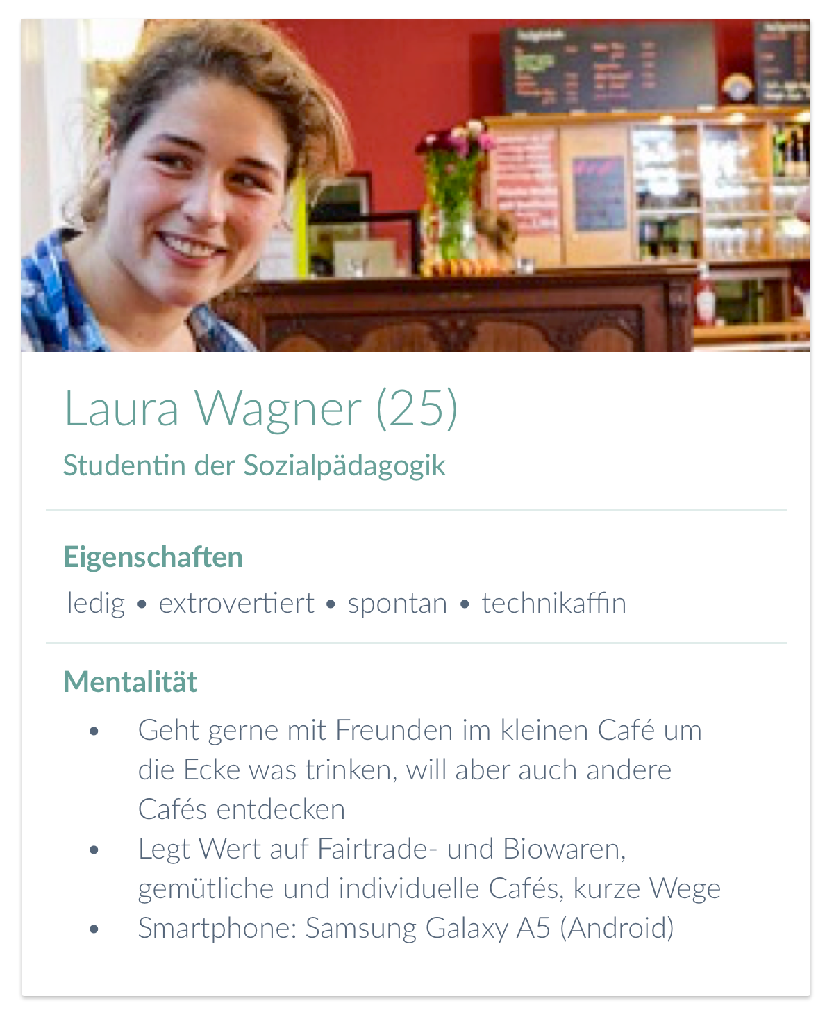
\includegraphics[width=0.5\textwidth]{Bilder/laura.eps}
		\caption{Primärpersona Laura Wagner}
		\label{fig:laura}
\end{figure}

\subsection{Sekundärpersona}
Roland Reisenweber vertritt die sekundäre Zielgruppe (vgl. Abb. \ref{fig:roland}). Er...
\begin{itemize}
	\item ...ist 42 Jahre alt
	\item ...ist verheiratet
	\item ...arbeitet als Journalist bei Frankfurter Allgemeine
	\item ...ist extrovertiert und offen für Neues
	\item ...arbeitet gerne an öffentlichen Orten
	\item ...besitzt ein ausgeprägtes soziales Bewusstsein
	\item ...ist gerne mit seiner Frau auf Reisen (innerhalb der EU)
	\item ...will regionale Kulturen kennenlernen
	\item ...ist weniger technikaffin, d. h. er nutzt sein iPhone nur zum telefonieren
\end{itemize}

\begin{figure}[h!]
    \centering
		
\includegraphics[width=0.5\textwidth]{Bilder/roland.eps}
		\caption{Sekundärpersona Roland Reisenweber}
		\label{fig:roland}
\end{figure}

\section{Anforderungsanalyse}
In der Anforderungsanalyse haben wir die Muss-, Soll- und Kann-Anforderungen von comfycoffee definiert.

\underline{Learnings:}
Dabei war die Herausforderung, die Anforderungen exakt zu formulieren und in Pakete zu unterteilen, die klein genug waren, um sie in der im Ablaufplan definierten Zeit abzuarbeiten (vgl. Kapitel \ref{sec:ablaufplan}).


\subsection{Muss-Anforderungen}
\label{subsec:mussanforderungen}
Die Muss-Anforderungen wurden auf das Nötigste heruntergebrochen, um die App sinnvoll bedienen zu können. Vorgabe war, den Bewegungssensor (Gyroskop) und GPS zu benutzen. Daraus ergaben sich die folgenden Muss-Anforderungen:

\begin{itemize}
	\item Lokale Cafés in der Nähe anzeigen
	\item Kartenansicht in Google Maps
	\item Listenansicht der Cafés im Umkreis
	\item Standortdaten via Google API
	\item Kaffeelexikon
	\item Einträge über Zubereitungsarten
	\item Schüttelfunktion (Benutzung des Bewegungssensors) für Zufallswahl einer Zubereitungsart
\end{itemize}

\subsection{Soll-Anforderungen}
Die Soll-Anforderungen erweitern den Funktionsumfang der App um nützliche Inhalte. Diese waren:

\begin{itemize}
	\item Navigation zu ausgewähltem Café über die App \emph{Google Maps}
	\item Listenansicht mit den wichtigsten Standortinformationen
	\item Detailseite mit mehr Infos über das Café (die Informationen sind abhängig davon, was die Google API zur Verfügung stellt)
\end{itemize}

\subsection{Kann-Anforderungen}
Die Kann-Anforderungen ergänzen die App durch weitere Informationen und Features, die der Nutzer nicht zwingend erwartet, aber als angenehm empfindet. Die Kann-Anforderungen waren:

\begin{itemize}
	\item Mehr Daten über zusätzliche APIs
	\item Eigene Bewertungen der Cafés durch die App
	\item Eigene Standorte vorschlagen
	\item Erweitertes Lexikon (z. B. mit Kaffeesorten, etc.)
	\item Profil des Nutzers anlegen
\end{itemize}


\section{Ablaufplan}
\label{sec:ablaufplan}
Anschließend wurde ein Ablaufplan (vgl. Abb. \ref{fig:ablaufplan}) ausgearbeitet und festgelegt. Dabei sollte die Designphase mit Wireframes, Flow Charts, MockUps und einem interaktiven Prototyp bis zum 22.11.2017 abgeschlossen sein. Für die Einarbeitung in das Entwicklungsframework, React Native (vgl. Kapitel \ref{sec:reactnative}), wurde eine Woche eingeplant. Bis zum 29.11.2017 sollte eine ``Hello World''-Anwendung laufen, um die Grundzüge des Frameworks zu beherrschen. Zwei Wochen, also bis zum 13.12.2017, waren für die Muss-Anforderungen, eine Woche für die Soll-Anforderungen (bis 20.12.2017) geplant. Die Kann-Anforderungen sollten im Januar 2018 abgeschlossen sein. Das folgende Diagramm veranschaulicht den Ablauf.\newline

\begin{figure}[h!]
    \centering
		
\includegraphics[width=\textwidth]{Bilder/ablaufplan.png}
		\caption{Ablaufplan der Konzeption und Entwicklung von comfycoffee}
		\label{fig:ablaufplan}
\end{figure}

\underline{Learnings:}
Die Aufwandsschätzung zu Beginn gestaltete sich als schwierig, da keine Erfahrung mit React Native und der Cross-Plattform-Entwicklung bzw. allgemein der App-Entwicklung vorhanden war.

\section{Flow Chart}
Das Flow Chart stellt die Navigation durch die App und die verschiedenen Views dar (vgl. Abb. \ref{fig:flowchart}). Von der Startseite aus kann der Nutzer wählen, ob er die Karte mit den Cafés in der Nähe oder das Kaffee-Lexikon aufrufen will.

In der Karte befindet sich eine Bottom Navigation Bar, mit der von der Karte zur Listenansicht und zurück gewechselt werden kann. Klickt der Nutzer in der Karte auf einen Marker oder in der Liste auf einen Eintrag, so wird er auf die Detailseite des jeweiligen Café geleitet. Dort erhält er Informationen wie Adresse, Öffnungszeiten und Bewertungen des Cafés. Über einen Button wird die Navigation zu dem Café in Google Maps geöffnet. Das Navigationskonzept wurde in der Entwicklung abgeändert, um den Design-Guidelines von Android und iOS zu entsprechen. Aus der Bottom Navigation Bar wurde in Android eine Tab Bar. Weiterhin wird auf der Detailseite eine Tab bzw. Bottom Navigation Bar angezeigt, um von der Seite des Cafés zu den Bewertungen zu wechseln.

Das Lexikon beinhaltet verschiedene Kaffeesorten. Beim Auswählen einer Kaffeesorte wird der Nutzer auf eine Unterseite geleitet, die Details zu der jeweiligen Kaffeesorte enthält. Schüttelt der Nutzer das Smartphone, während er sich auf der Übersichtsseite des Lexikons befindet, wird zufällig eine Kaffeesorte ausgewählt und der Nutzer hat die Möglichkeit, sich zu der genannten Detailseite navigieren zu lassen.\newline

\begin{figure}[h!]
    \centering
		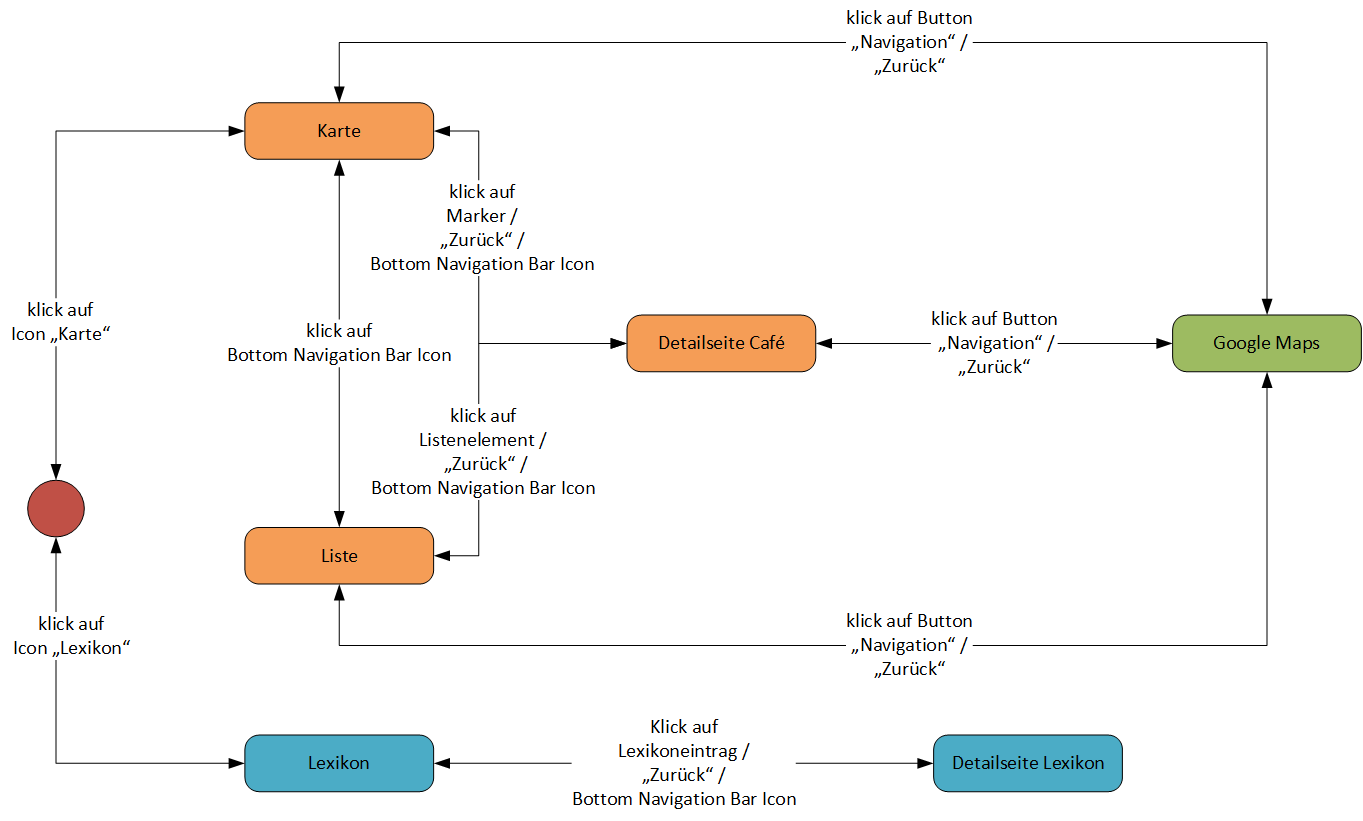
\includegraphics[width=\textwidth]{Bilder/flowchart.png}
		\caption{Erster Entwurf des Flow Charts von comfycoffee}
		\label{fig:flowchart}
\end{figure}

\newpage

\section{Wireframes}
Nachdem die Anzahl und Anforderungen an die Views feststanden, wurden diese auf Papier in Form von Wireframes visualisiert. Dabei wurden die Elemente pro View bestimmt und deren Position auf den einzelnen Seiten festgelegt (vgl. Abb. \ref{fig:wireframes}).

\begin{figure}[h!]
    \centering
		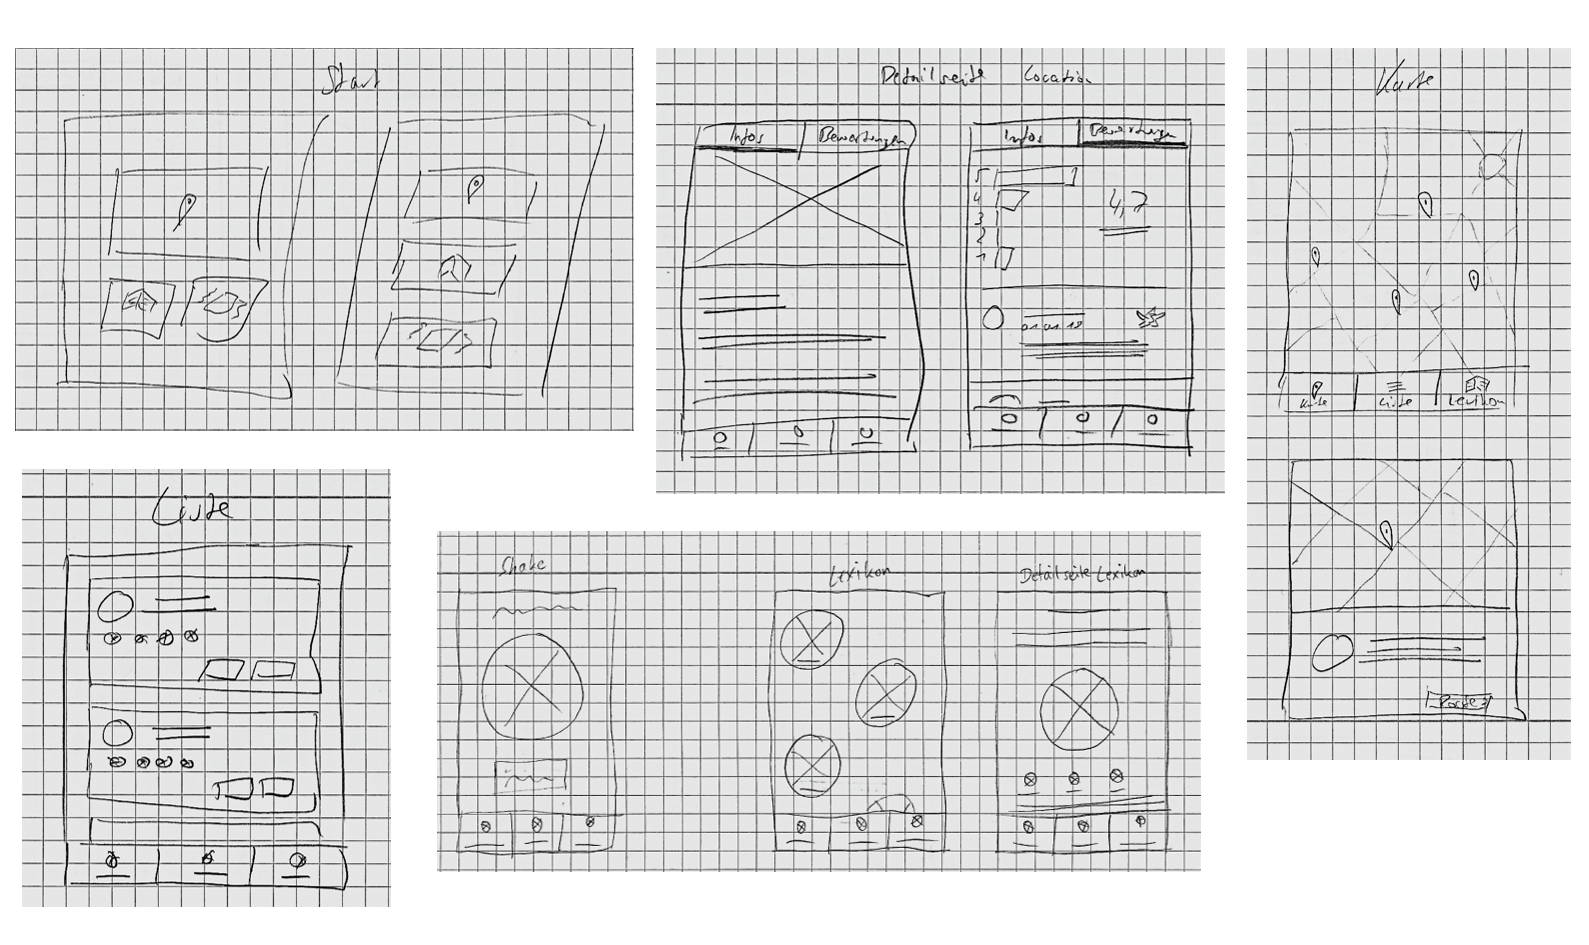
\includegraphics[width=\textwidth]{Bilder/wireframes.png}
		\caption{Wireframes von comfycoffee}
		\label{fig:wireframes}
\end{figure}

\newpage
\section{MockUps}
Aus den Wireframes wurden MockUps mit dem MockUp-Tool Axure konfiguriert. Zu jeder View wurde ein MockUp erstellt. Im Gegensatz zu den Wireframes sind hier schon Farben, Bilder und Texte beispielhaft enthalten (vgl. Abb. \ref{fig:mockup}).\newline

\begin{figure}[h!]
    \centering
		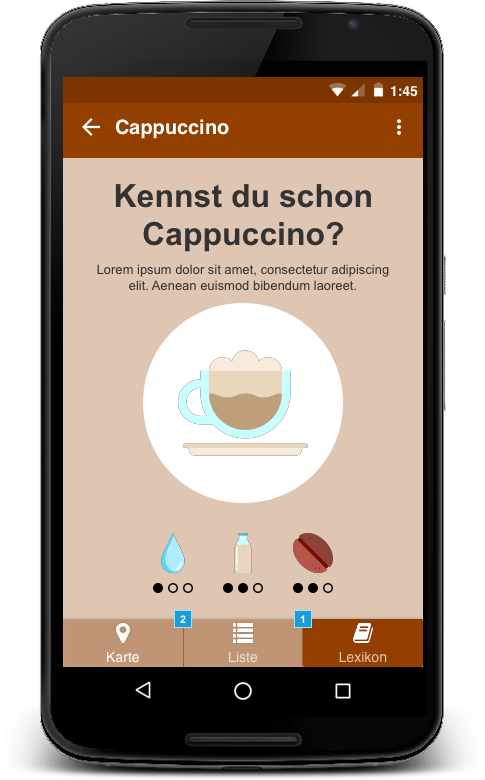
\includegraphics[width=0.5\textwidth]{Bilder/detail.png}
		\caption{Ansicht der Detailseite eines Kaffees als MockUp}
		\label{fig:mockup}
\end{figure}

\section{Prototyp}
Anhand der MockUps und des Flow Charts wurde in Axure ein interaktiver Prototyp erstellt. Er dient zum Durchklicken durch die App und um einen ersten Eindruck in Sachen Usability zu gewinnen. Der Prototyp ist online verfügbar unter\newline \url{https://jzd0d2.axshare.com}.



\chapter{Entwicklung}
\label{entwicklung}
Mit dem Abschluss der Konzeptionsphase begann die technische Umsetzung der App.
Nachdem ein passendes Framework zur Entwicklung der App auf mehreren Plattformen gefunden wurde, konnte eine sinnvolle Projektstruktur mit allen benötigten Bibliotheken angelegt werden.
Die Implementierung einiger Freatures wurde dabei parallel durchgeführt.
Weiterhin wird in diesem Kapitel der aktuelle Stand der App beschrieben.
Eine Readme inklusive Installationsanleitung schließt die technische Seite des Projekts ab.

\section{React Native}
\label{sec:reactnative}
Nach kurzer Diskussion und dem Abwägen von Vor- und Nachteilen entschieden wir uns dafür, das \emph{React Native} Framework zu benutzen.
React Native stellt somit das technische Kernelement des Projekts dar.
Als ein von \emph{Facebook} entwickeltes und verwaltetes Repository erfreut es sich mit über 58.000 Sternen auf \emph{GitHub} großer Beliebtheit.
Demnach steht bereits eine große Community hinter dem Cross-Plattform-Framework.
Die Entwicklung mit React Native erfolgt fast ausschließlich über JavaScript.
Als Cross-Plattform-Framework ermöglicht React Native den Zugriff auf native Komponenten via JavaScript und profitiert somit von einer besseren Performance als hybride Frameworks.
Allerdings erscheint es trotz seiner Popularität technisch noch nicht sehr etabliert.
Darüber hinaus benötigen die nativen Komponenten meist noch Anpassungen per Hand für Android und iOS.

\section{Setup}
Um React Native einem Projekt hinzuzufügen stehen zwei Möglichkeiten zur Verfügung.
Eine davon ist der \emph{Quick Start}, welcher nach erfolgreichem Ausführen einen QR-Code anzeigt.
Über das Smartphone kann der Code gescannt und die App aufgerufen werden.
Vor- und Nachteil gleichermaßen ist, dass die Entwicklungsumgebungen \emph{Android Studio} für Android und \emph{Xcode} für iOS nicht installiert sein müssen.
Allerdings ist es somit auch nicht möglich, selbsterstellte React Native Module hinzuzufügen.
Demnach entschieden wir uns für die zweite Variante, um zusätzlich Zugriff auf eigene Module zu haben.
Hierbei wird React Native über die Kommandozeile und den Befehl 'create-react-native-app' initialisiert.

Grundvoraussetzungen hierbei sind eine funktionierende Version von \emph{Node.js} sowie das Facebook Tool \emph{Watchman}.
Für die Verwaltung von Abhängikeiten wird bei der Installation von React Native der Paketmanager \emph{Yarn} hinzugefügt, der Zugriff auf die über den \emph{Node Package Manager (npm)} bereitgestellten Module ermöglicht.
Zusätzlich müssen die beiden Entwicklungsumgebungen Android Studio und Xcode zum Kompilieren des nativen Codes bereit stehen.
Testing und Debugging der App kann somit entweder über die in Android Studio und Xcode integrierten Simulatoren erfolgen oder aber direkt über ein verbundenes Smartphone.

Unsere Wahl für einen Code Editor fiel auf \emph{Visual Studio Code} von Microsoft, da es einen einfachen Einstieg bietet und sowohl für Windows als auch für Mac verfügbar ist.
Als Versionierungssystem benutzten wir Bitbucket, welches die Verwaltung von Git-Repositories ermöglicht.
Des Weiteren richteten wir ein \emph{Trello-Board} ein, auf dem das Projektmanagement abgebildeten werden sollte.

\underline{Learnings:}
Obwohl die Konzeption unserer App auf einen eher geringen Umfang schließen lässt wurden doch sehr viele Tools benötigt, um eine Entwicklung zu ermöglichen.
Für diese Projektgröße stellte sich auch das Projektmanagement-Tool Trello als zu aufwändig in der Pflege heraus.



\section{Module}
Für die Implementierung einiger Funktionalitäten stehen bereits zahlreiche Komponenten und Pakete aus der Community zu Verfügung.
Zusätzlich zu den bereits in React Native integrieren Modulen werden folgende in der App verwendet:
\begin{itemize}
	\item \textbf{axios}: Erleichtert die Kommunikation mit beliebigen APIs, da es entsprechende Hilfmethoden zur Verfügung stellt.
	\item \textbf{react-native-maps}: Eine benutzerdefinierte React Native Komponente, welche die Integration einer Google Maps Karte ermöglicht. Leider ein sehr undokumentiertes Modul, welches große Probleme bei der Integration aufwirft.
	\item \textbf{react-native-permissions}: Bietet eine Schnittstelle zur Abfrage von unterschiedlichen Berechtigungen, beispielsweise dem Zugriff auf den aktuellen Standort.
	\item \textbf{react-native-sensors}: Ermöglicht den direkten Zugriff auf den Bewegungssensor des entsprechenden Endgeräts - leider ein ebenfalls eher undokumentiertes Modul.
	\item \textbf{react-native-star-rating}: Die visuelle Darstellung eines Werts (wie beispielsweise einer Bewertung) in Form von Sternen verpackt in einer React Native Komponente.
	\item \textbf{react-native-vector-icons}: Eine Sammlung thematisch geordneter Icon-Bi\-blio\-theken, welche nach dem Import direkt zur Verfügung stehen.
	\item \textbf{react-navigation}: Ein alternatives Navigationskonzept als React Native Modul aus der Community. Dieses ersetzt das in React Native integrierte Konzept und ermöglicht eine einfache Implementierung diverser Navigationselemente.
\end{itemize}

Während der Entwicklung wurden einige zusätzliche Module eingebunden, welche allerdings nicht den gewünschten Anforderungen entsprachen:
\begin{itemize}
	\item \textbf{react-native-material-bottom-navigation}: Die ebenfalls in den Material Design Guidelines vertretene Bottom Navigation für Android verpackt in einer React Native Komponente. In dieser App wird allerdings die Navigation in Android über Tabs bevorzugt.
	\item \textbf{react-native-stars}: Eine Alternative zu dem verwendeten react-native-star-rating Modul. Da dieses Modul weniger Konfigurationsmöglichkeiten bietet als sein Pendant ist es obsolet.
	\item \textbf{react-native-google-places-autocomplete}: Die reduzierte Variante des react-native-maps Moduls. Allerdings ist der Funktionsumfang deutlich zu gering, so bietet es lediglich autocomplete für die Google Places API.
\end{itemize}

Durch die zahlreichen verfügbaren Komponenten lässt sich eine React Native App sehr stark modularisieren.
Es können bei Bedarf die jeweils benötigen Funktionalitäten isoliert angefordert und eingebunden werden.
Einzig undokumentierte und redundante Module stellen einen zusätzlichen Aufwand dar.
Diese müssen zunächst herausgefiltert und getestet werden, um die beste Lösung zu finden.

\section{Arbeitsaufteilung}
Die Aufteilung der anstehenden Aufgaben sahen wir als notwendig an, um die geplanten Deadlines einhalten zu können.
Unumgänglich war allerdings eine gemeinsame Code-Basis, in die zusätzliche Funktionalitäten unabhängig voneinander integriert werden konnten.
Hierzu legten wir durch \emph{Pair Programming} zusammen eine geeignete Grundlage.

\subsection{Gemeinsame Aufgaben}
Das Fundament besteht aus dem Grundgerüst der App sowie der Navigation durch diese.
Dabei besteht das Navigationskonzept aus einer übergeordneten \emph{Stack Navigation} sowie mehreren kontextabhängigen, verschachtelten \emph{Tab/Bottom Navigations}.
Eine dem Flow Chart entsprechende Seitenstruktur ermöglicht es, Seiteninhalte isoliert zu bearbeiten.
Die Implementierung der Karte wurde ebenfalls gemeinsam gelöst, allerdings nach Betriebssystemen getrennt.
Sobald der Rahmen der App aufgebaut war arbeiteten wir an unterschiedlichen Funktionalitäten weiter.

\underline{Learnings:}
Bereits in diesem frühen Stadium konnten wir einige Aha-Momente für uns entdecken.
Die Tabs und Bottom Navigation, so wie in unseren MockUps skizziert, ließ sich nur teilweise realisieren.
Eine weitere Recherche ergab, dass der Aufbau der Navigation in React Native eine andere Lösung für diesen Fall vorgab und wir die Implementierung entsprechend anpassen mussten.
Darüber hinaus stießen wir mit dem React Native Modul für die Google Maps Karte (react-native-maps) bereits auf ein undokumentiertes Modul aus der Community, welchem noch Weitere folgen sollten.

\subsection{Aufgaben von Katharina Garrecht}
Die Umsetzung der Inhalte des Lexikons und der Lexikon-Detailansicht sowie die Integration des Bewegungssensors übernahm Katharina Garrecht.
Hierbei implementierte sie die im Prototypen definierten Elemente sowohl für die Übersichtsseite als auch für das Template der Kaffee-Detailseite.
Die Detailseiten werden dabei mit in einer JSON Datei hinterlegten Inhalten gespeist.
Auf der Übersichtsseite selbst ist der Bewegungssensor aktiv, welcher bei Erkennung einer Schüttelgeste zufällig eine der zur Verfügung stehenden Kaffee-Zubereitsungsarten auswählt und vorschlägt.

\underline{Learnings:}
Die Integration des Bewegungssensors in die bestehende Navigation brachte einige Stolpersteine mit sich, die nur durch lange Recherchen und Umwege überwunden werden konnten.
Auch die Einarbeitung in native UI Komponenten der jeweiligen Betriebssysteme war für die Umsetzung dieser Funktionalitäten notwendig.

\subsection{Aufgaben von Thomas Wedler}
Die Darstellung der Listenansicht aller nahen Cafés sowie die Detailansicht einzelner Cafés fiel in den Aufgabenbereich von Thomas Wedler.
Ebenso Teil dieses Bereichs war die Implementierung der Geolocation zur Ermittlung des aktuellen Standorts.
Über diese Geokoordinaten werden bei Bedarf die \emph{Google Places API} und auch die \emph{Google Maps API} angesprochen.
Das Ergebnis ist situationsabhängig entweder eine Liste aller umliegenden Cafés mit rudimentären Informationen zu diesen oder aber ein ausführliches Objekt mit zahlreichen Detailinformationen über ein einzelnes Café.

\underline{Learnings:}
Für die Umsetzung der benötigen Funktionalitäten war eine intensive Einarbeitung in das Ecosystem sowie die bereitgestellten Schnittstellen der Google APIs unumgänglich.
Ebenfalls hier mussten native UI Komponenten der jeweiligen Betriebssysteme korrekt identifiziert und implementiert werden.

\newpage

\section{Vorstellung der App}
Im Folgenden wir die App mit ihren Views vorgestellt.
\nopagebreak

\begin{table}[h!]
	\hskip-0.2cm\begin{tabular}{p{0.5\textwidth}p{0.5\textwidth}}
		\multicolumn{2}{p{\textwidth}}{\subsection{Startseite}} \\
		\multicolumn{2}{p{\textwidth}}{Der Einstiegspunkt der App. Von dort aus ist die Navigation zur Umkreissuche oder zum Lexikon möglich (vgl. Abb. \ref{fig:startios} und \ref{fig:startandroid}).\newline} \\
		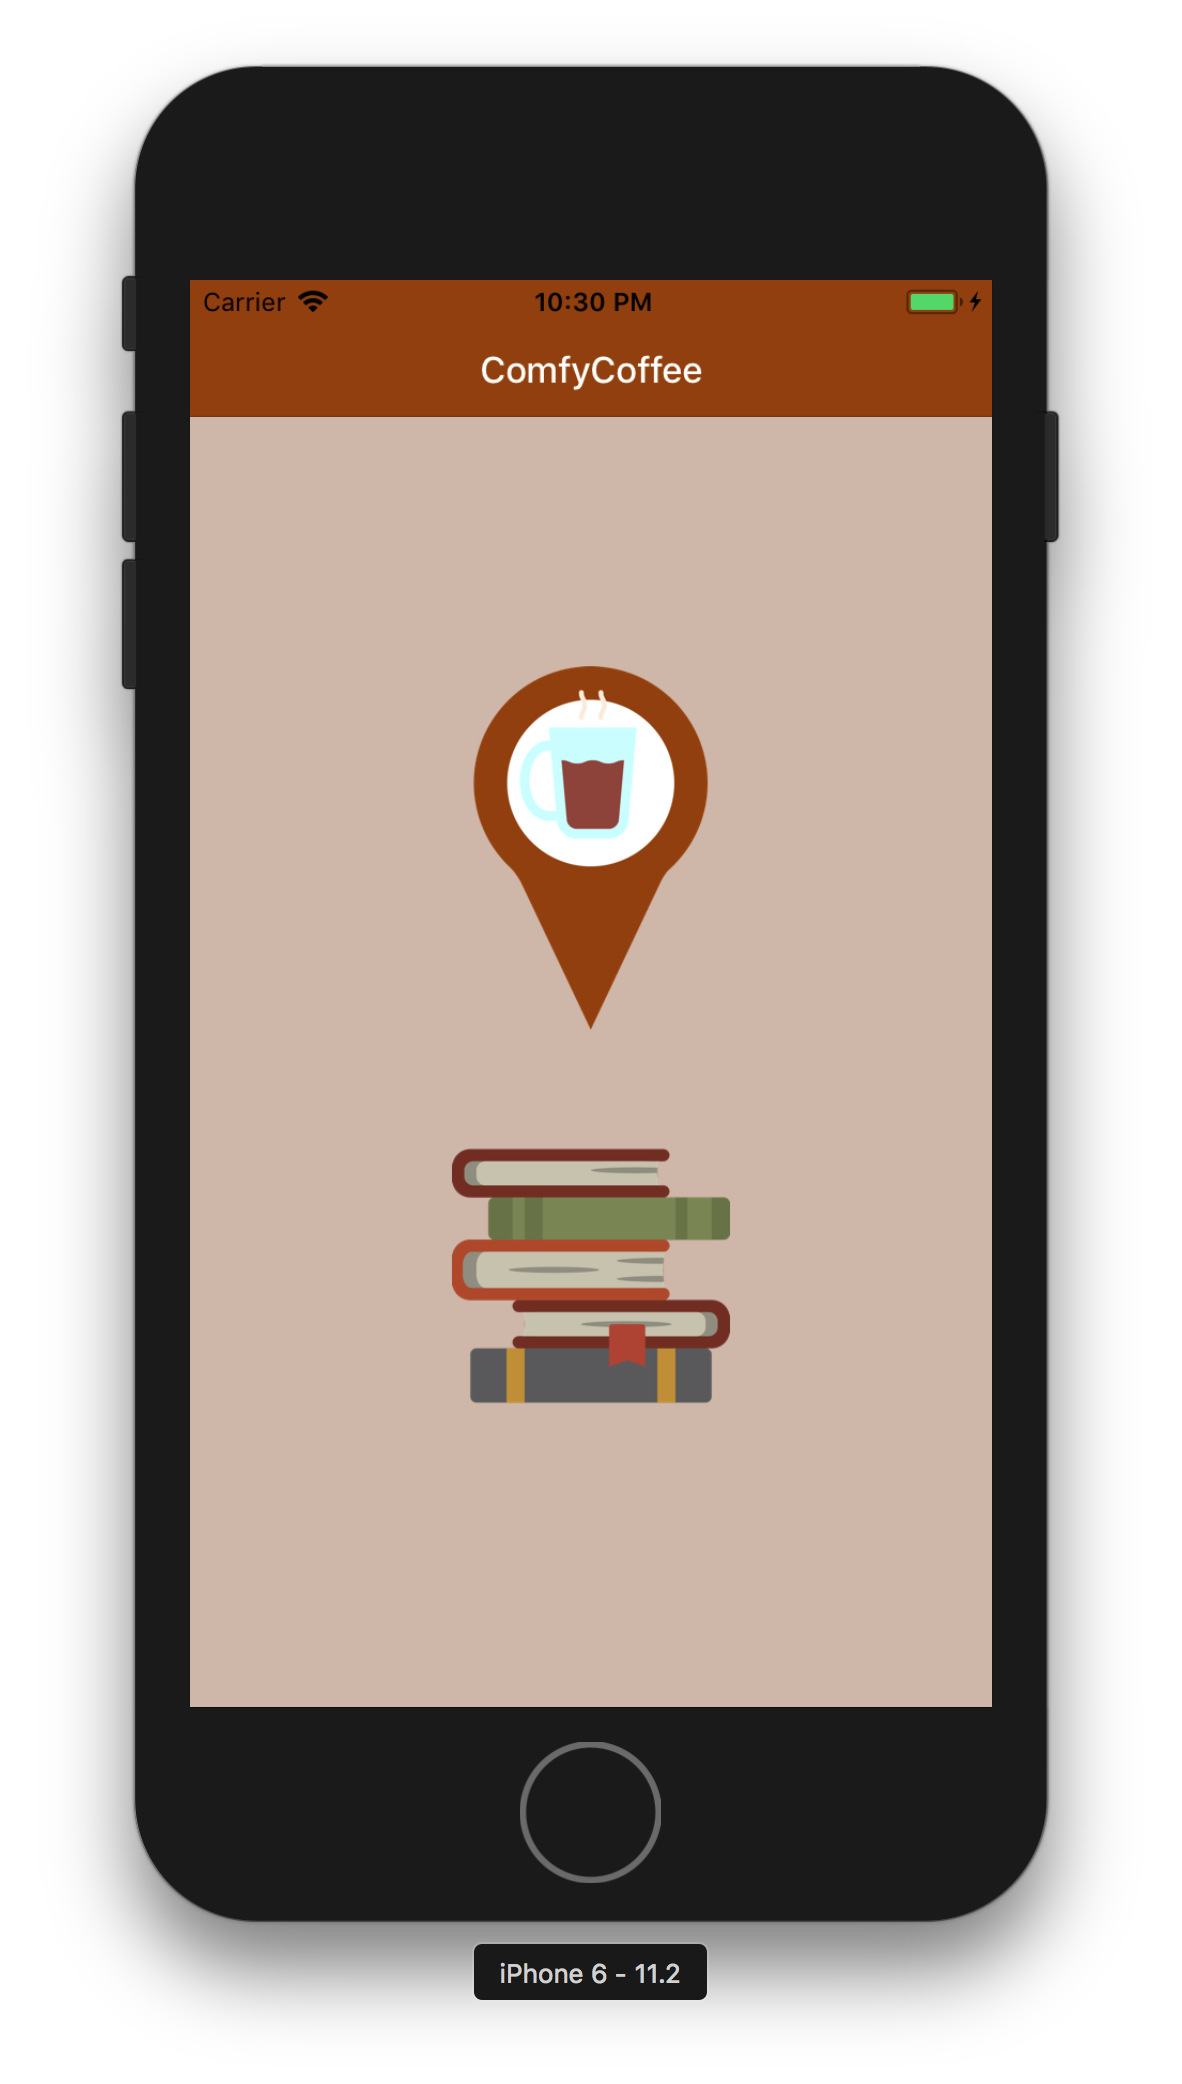
\includegraphics[width=0.5\textwidth]{Bilder/app-startseite.png}
		\captionof{figure}{Startseite der App unter iOS}
		\label{fig:startios} &
		\centering
		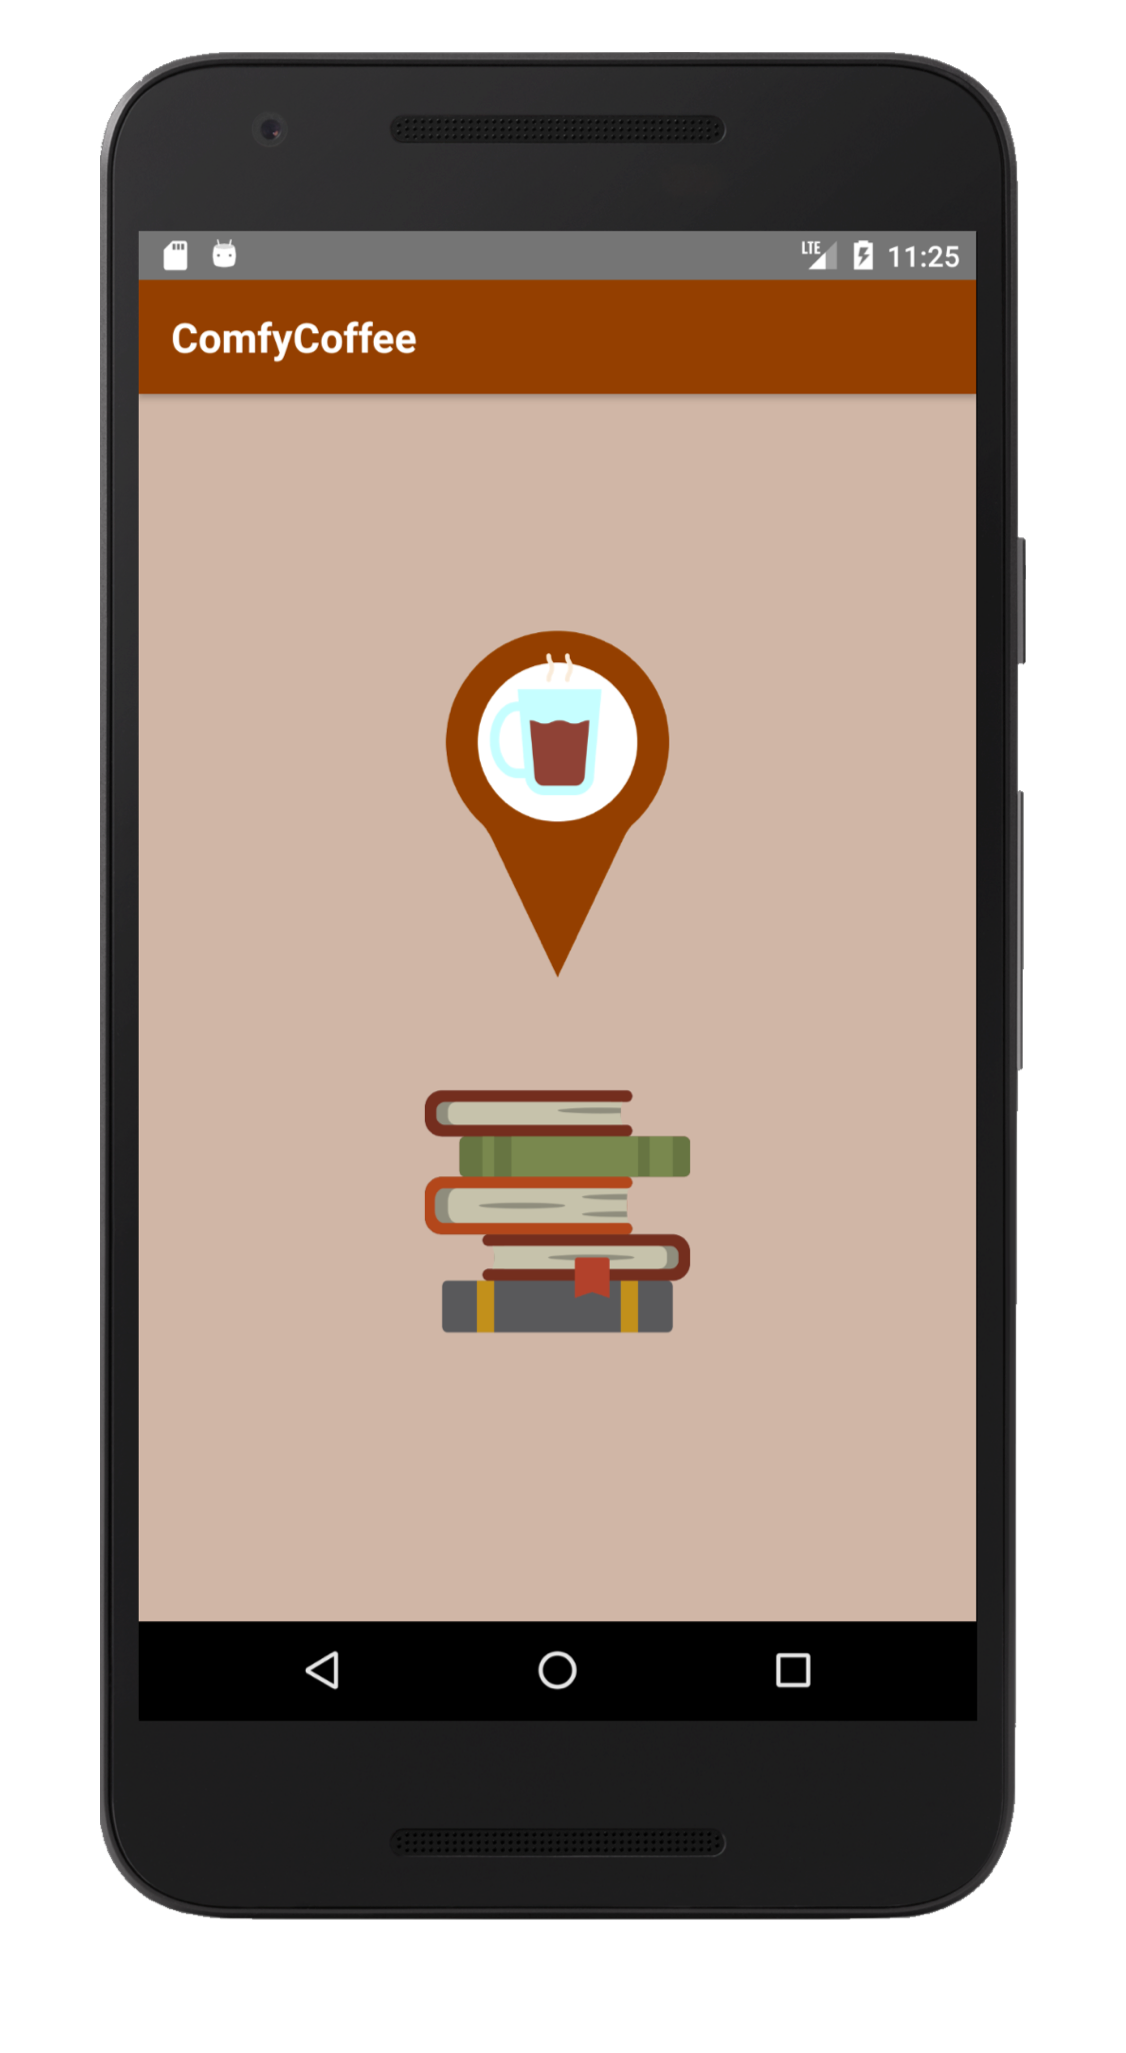
\includegraphics[width=0.48\textwidth]{Bilder/app-startseite_android.png}
		\captionof{figure}{Startseite der App unter Android}
		\label{fig:startandroid}
	\end{tabular}
\end{table}

\begin{table}
	\vskip-4.0cm\hskip-0.2cm\begin{tabular}{p{0.5\textwidth}p{0.5\textwidth}}
		\multicolumn{2}{p{\textwidth}}{\subsection{Kartenansicht}} \\
		\multicolumn{2}{p{\textwidth}}{Hier werden auf einer interaktiven Google Maps Karte alle sich in der Nähe befindlichen Cafés einschließlich des eigenen aktuellen Standorts angezeigt (vgl. Abb. \ref{fig:karteios} und \ref{fig:karteandroid}). Die hierfür benötigen Informationen werden über die entsprechenden Google APIs bezogen. Des Weiteren erreicht man von hier aus über die Tab Navigation in Android sowie die Bottom Navigation in iOS die Listenansicht der angezeigten Cafés.\newline} \\
		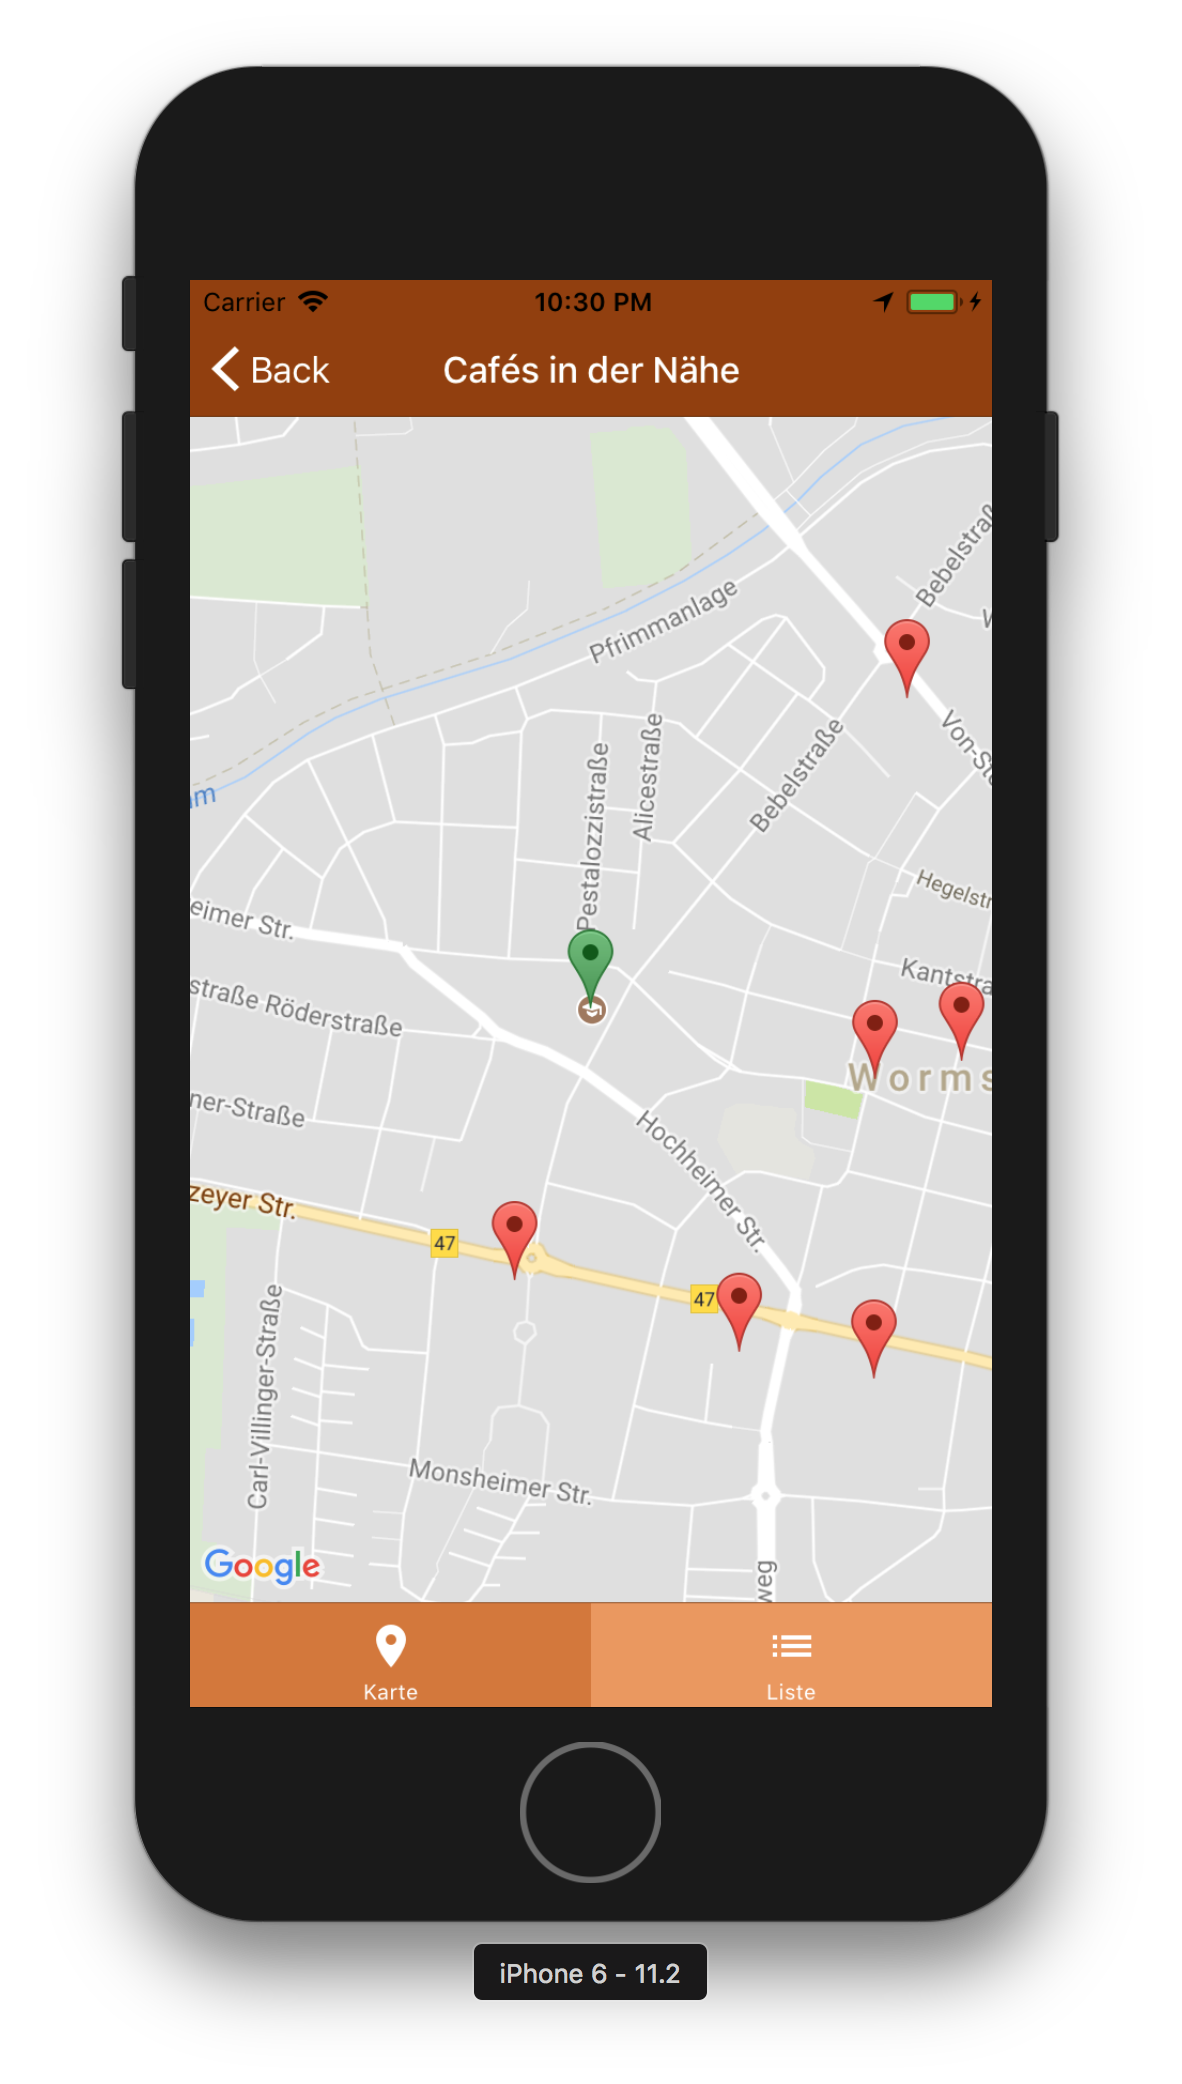
\includegraphics[width=0.5\textwidth]{Bilder/app-karte.png}
		\captionof{figure}{Kartenansicht der App unter iOS}
		\label{fig:karteios} &
		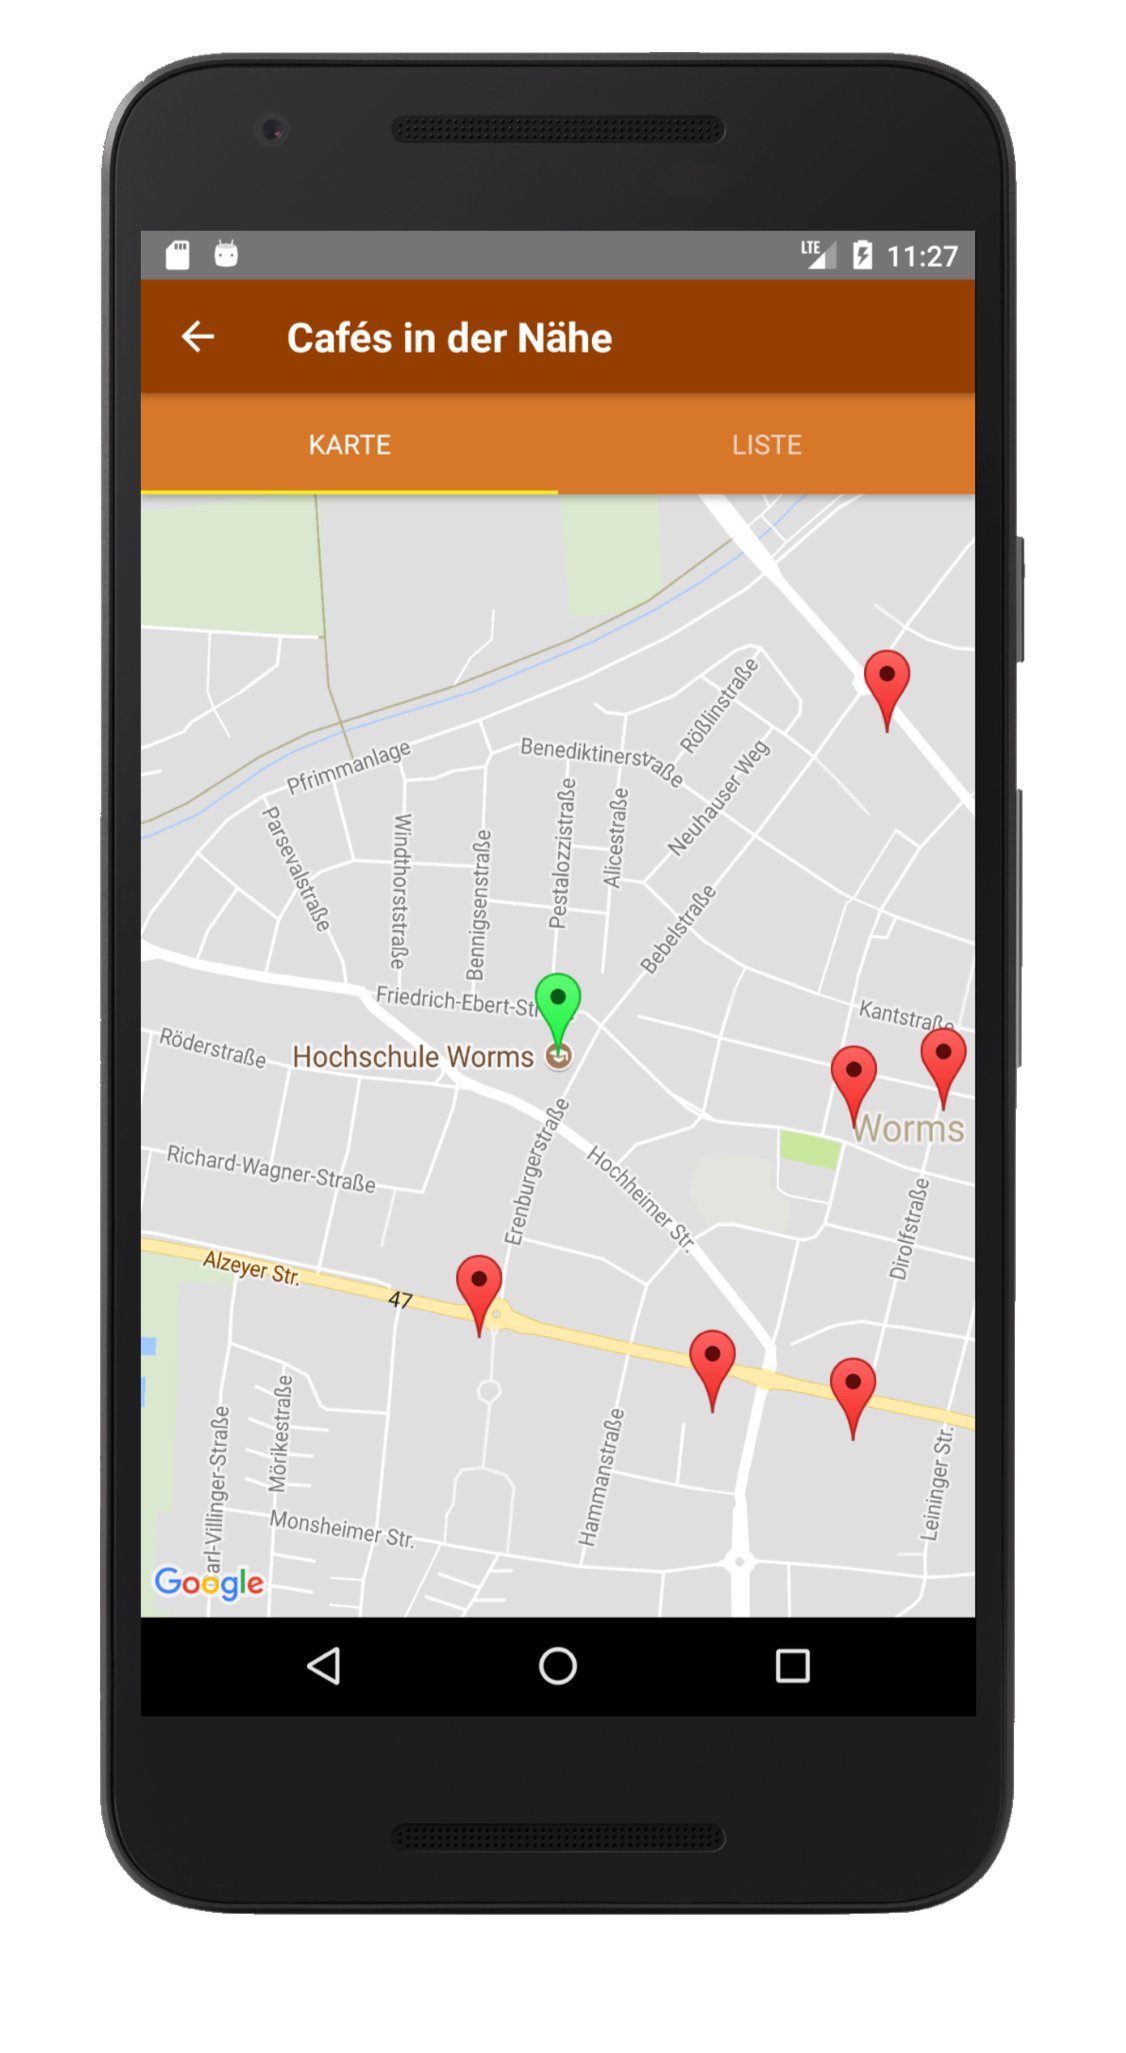
\includegraphics[width=0.48\textwidth]{Bilder/app-karte_android.png}
		\captionof{figure}{Kartenansicht der App unter Android}
		\label{fig:karteandroid}
	\end{tabular}
\end{table}

\begin{table}
	\vskip-4.0cm\hskip-0.2cm\begin{tabular}{p{0.5\textwidth}p{0.5\textwidth}}
		\multicolumn{2}{p{\textwidth}}{\subsection{Kartenansicht - ausgewählt}} \\
		\multicolumn{2}{p{\textwidth}}{Ein Klick auf einen Marker öffnet ein \emph{Bottom Sheet}, in welchem die wichtigsten Informationen über das ausgewählte Café wie etwa Entfernung, Bewertung, Öffnungszeiten oder Adresse angezeigt werden. Innerhalb dieses Sheets stehen Buttons zur Navigation auf die Detailseite des Cafés oder direkt zu Google Maps mit dem Café als hinterlegtem Ziel zur Verfügung (vgl. Abb. \ref{fig:karteiosactive} und \ref{fig:karteandroidactive}).\newline} \\
		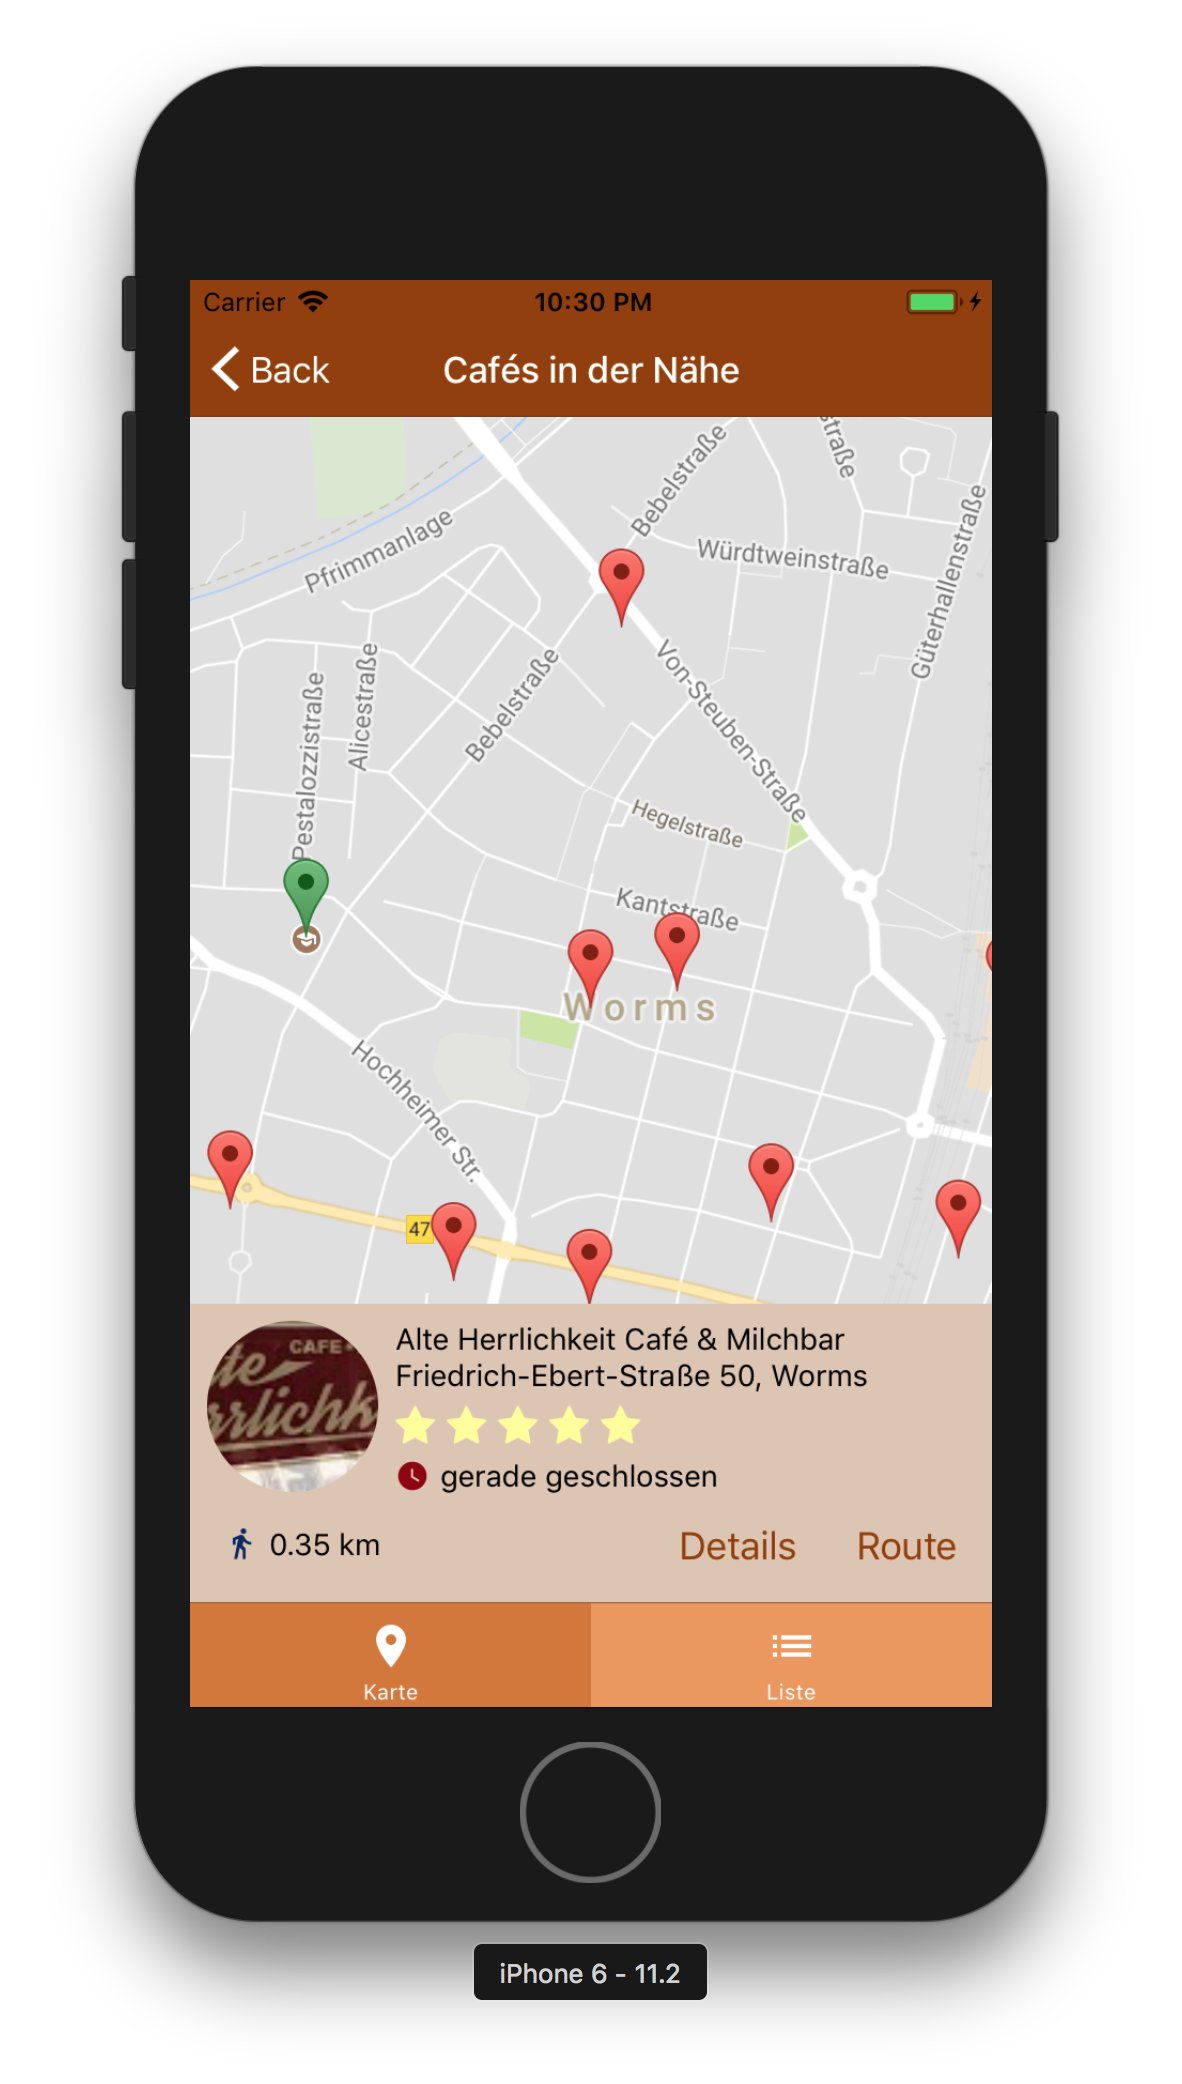
\includegraphics[width=0.5\textwidth]{Bilder/app-karte-active.png}
		\captionof{figure}{Kartenansicht (ausgewählt) der App unter iOS}
		\label{fig:karteiosactive} &
		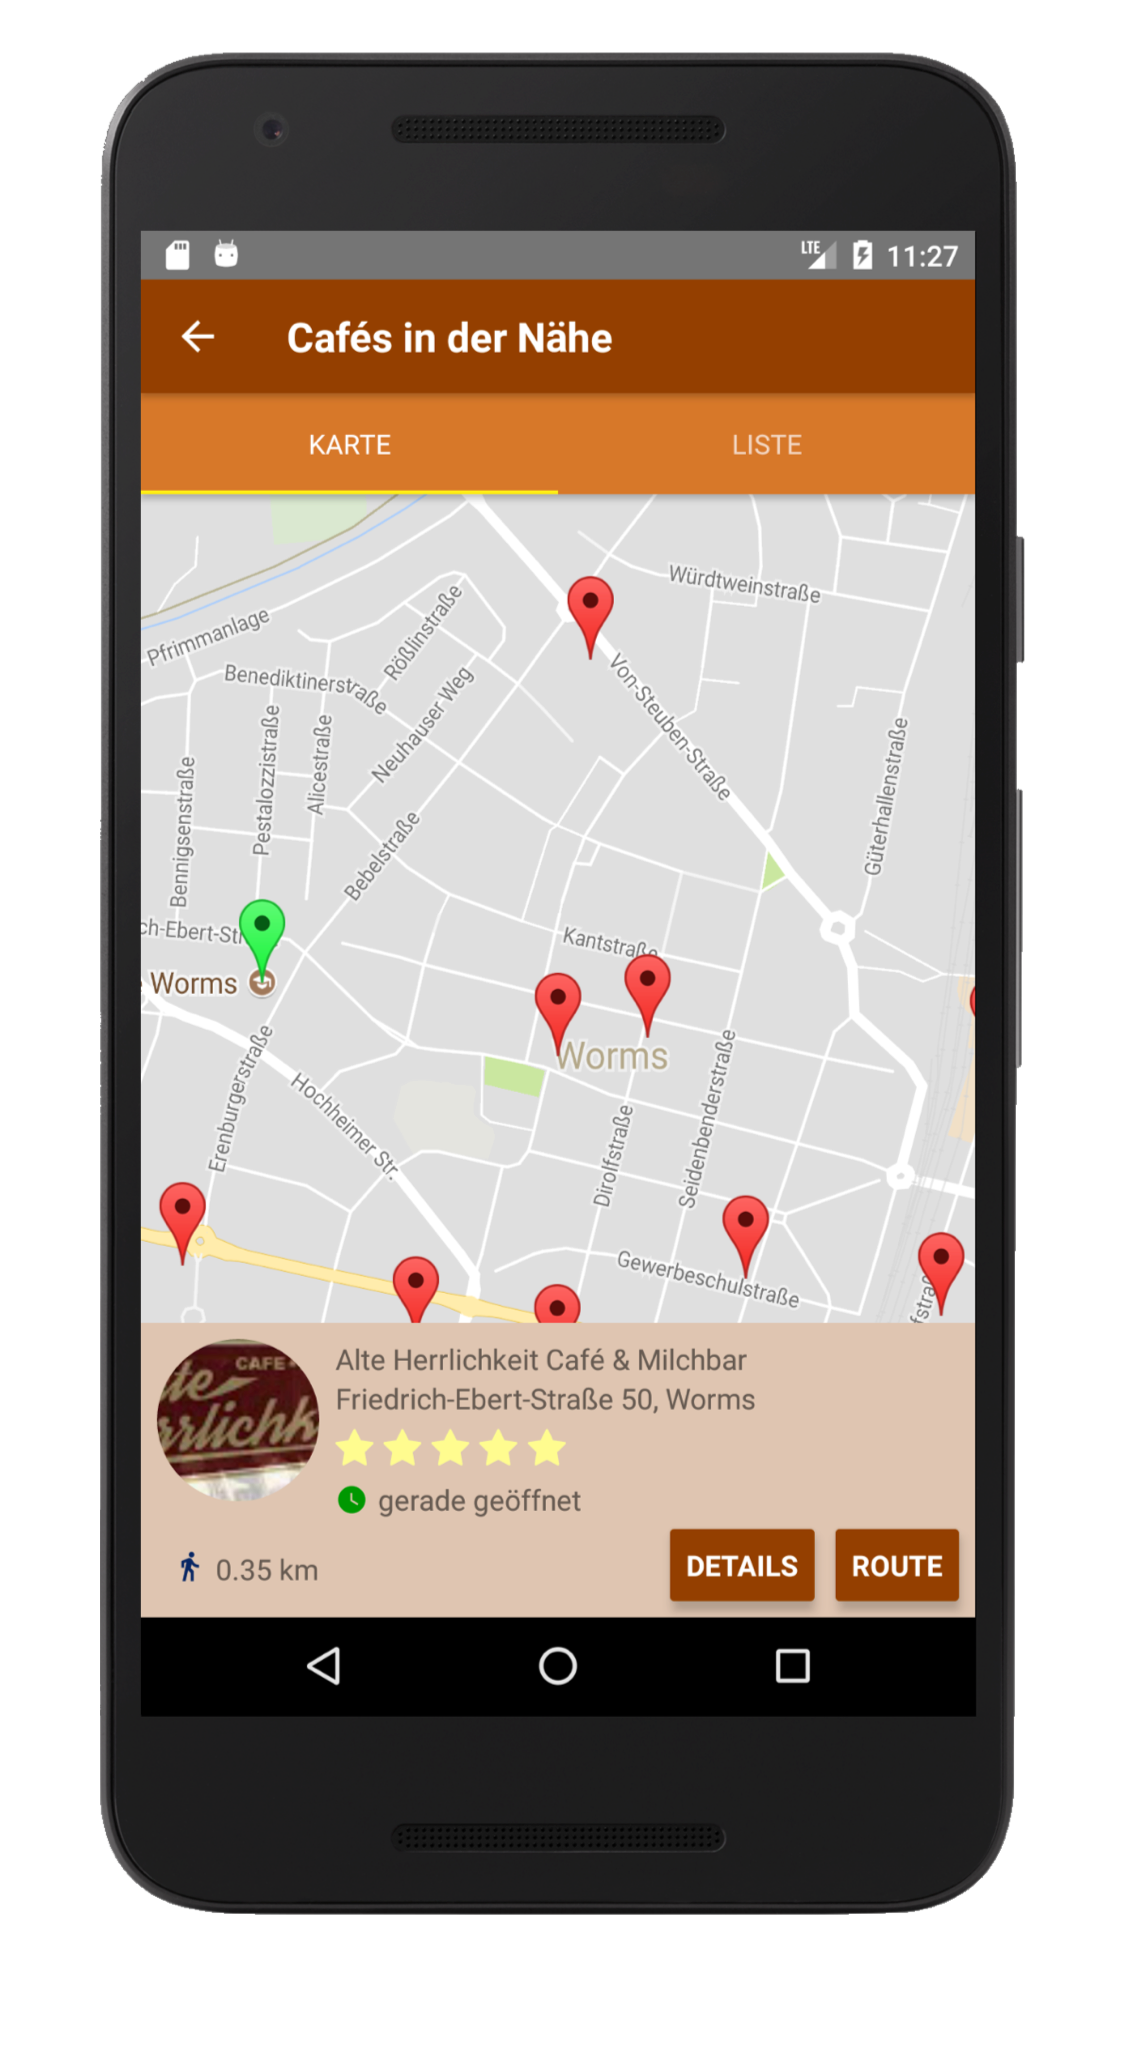
\includegraphics[width=0.48\textwidth]{Bilder/app-karte-active_android.png}
		\captionof{figure}{Kartenansicht (ausgewählt) der App unter Android}
		\label{fig:karteandroidactive}
	\end{tabular}
\end{table}

\begin{table}
	\vskip-4.0cm\hskip-0.2cm\begin{tabular}{p{0.5\textwidth}p{0.5\textwidth}}
		\multicolumn{2}{p{\textwidth}}{\subsection{Listenansicht}} \\
		\multicolumn{2}{p{\textwidth}}{Die bereits in der Kartenansicht dargestellten Standorte der Cafés werden hier in einer übersichtlichen Liste gezeigt (vgl. Abb. \ref{fig:listeios} und \ref{fig:listeandroid}). Jeder Listeneintrag enthält die gleichen Informationen und Interaktionsmöglichkeiten wie das Bottom Sheet aus der Karte, da es sich hierbei technisch um die gleiche, eigens konstruierte React Native Komponente handelt.\newline} \\
		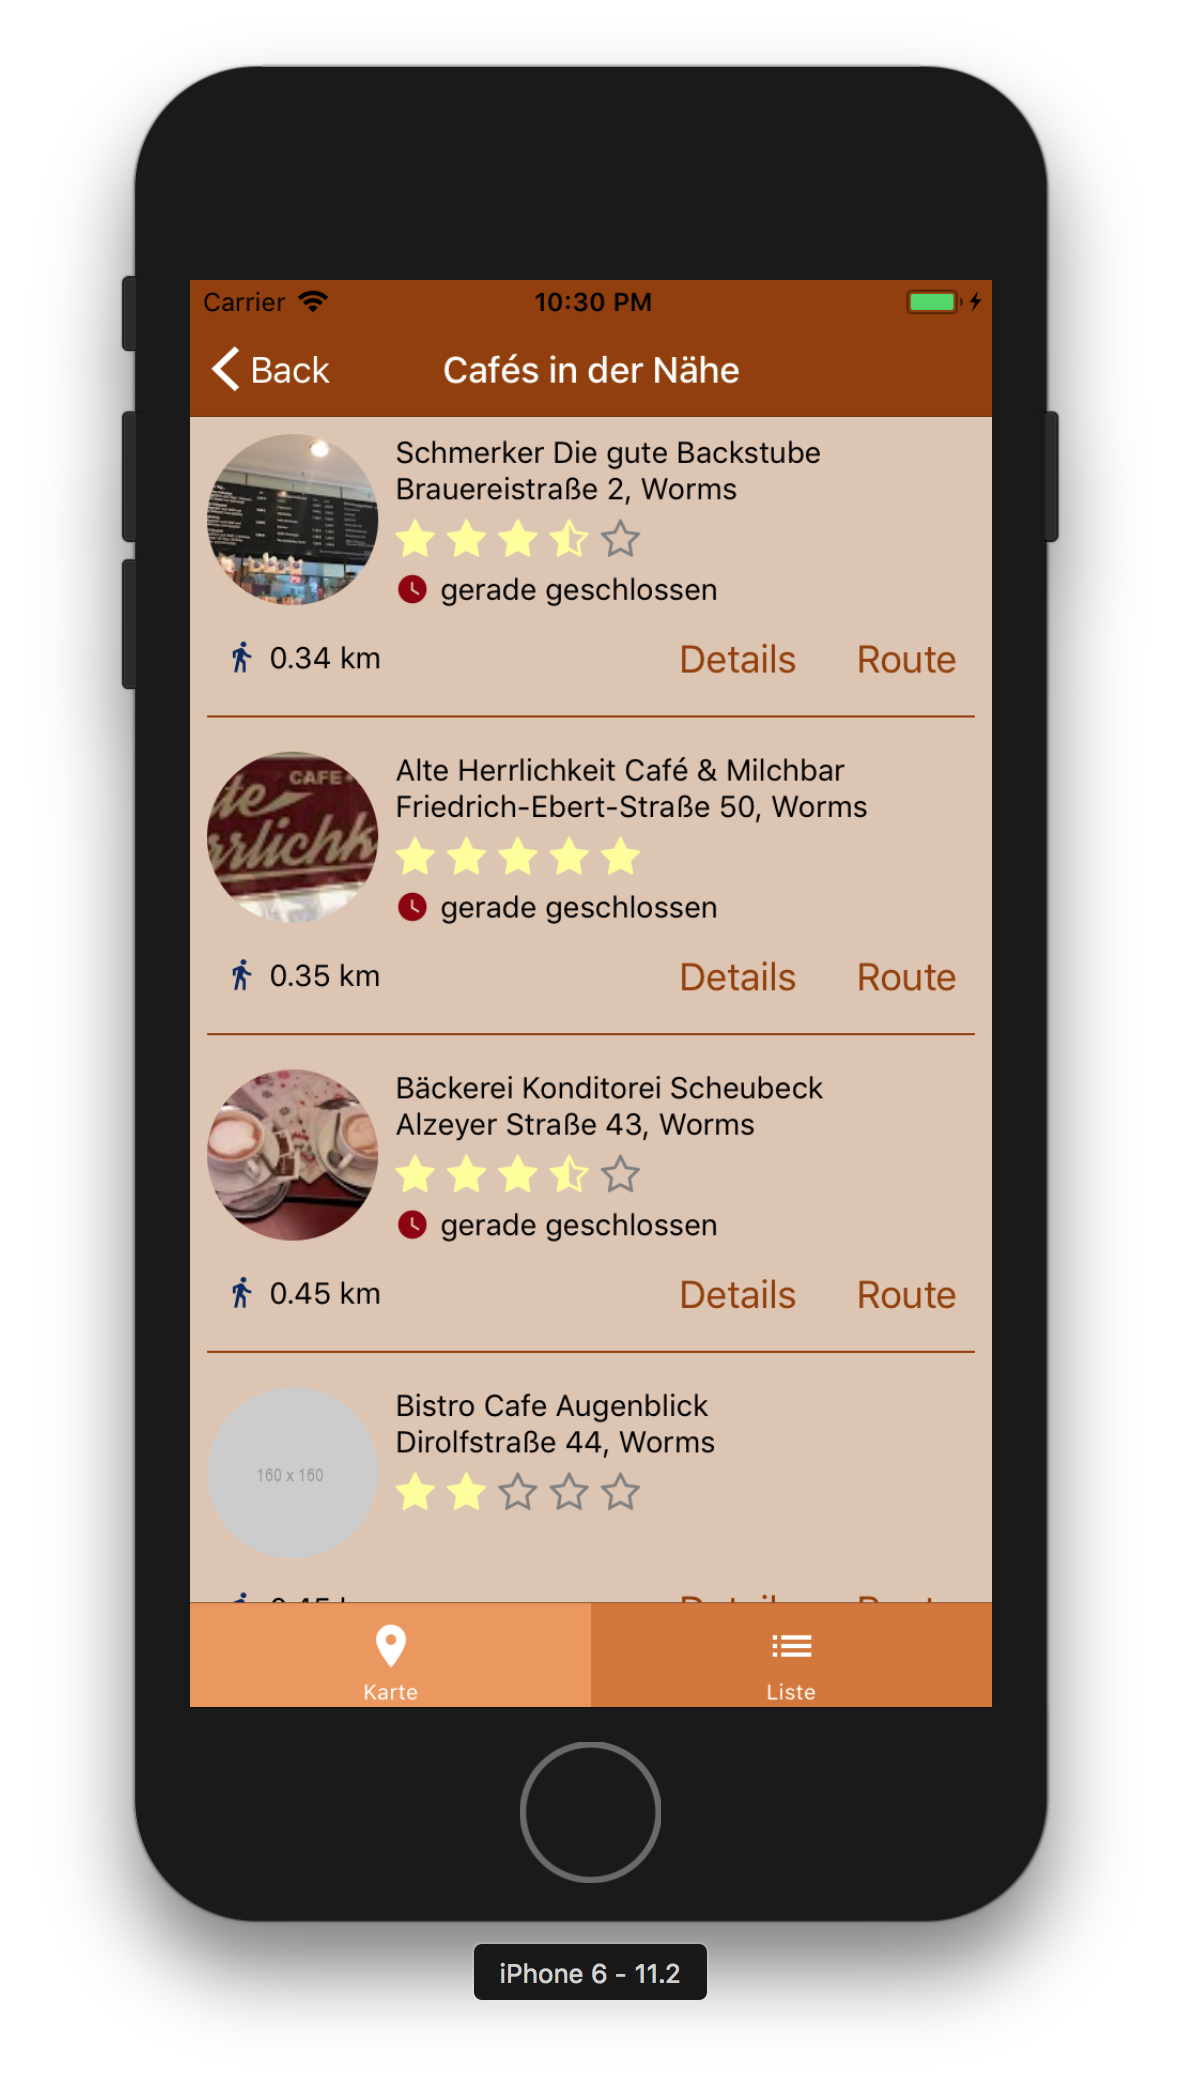
\includegraphics[width=0.5\textwidth]{Bilder/app-liste.png}
		\captionof{figure}{Listenansicht der App unter iOS}
		\label{fig:listeios} &
		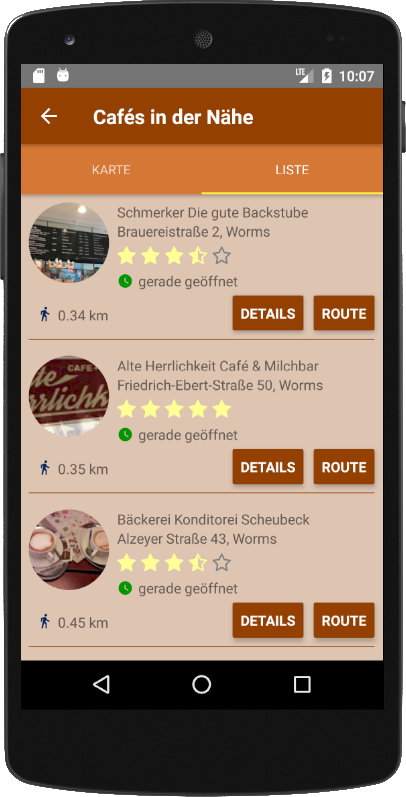
\includegraphics[width=0.48\textwidth]{Bilder/app-liste_android.png}
		\captionof{figure}{Listenansicht der App unter Android}
		\label{fig:listeandroid}
	\end{tabular}
\end{table}

\begin{table}
	\vskip-3.5cm\hskip-0.2cm\begin{tabular}{p{0.5\textwidth}p{0.5\textwidth}}
		\multicolumn{2}{p{\textwidth}}{\subsection{Infos Café}} \\
		\multicolumn{2}{p{\textwidth}}{Diese Seite zeigt die bereits im Bottom Sheet vorhandenen Informationen über das ausgewählte Café. Außerdem sind weitere Details wie Telefonnummer, Internetadresse oder auch Bilder des Cafés - soweit über die Google API bereit gestellt - verfügbar (vgl. Abb. \ref{fig:infoios} und \ref{fig:infoandroid}). Auch hier erreicht man über einen Button das Café als Zieladresse direkt in Google Maps. Darüber hinaus enthält die Tab Navigation respektive Bottom Navigation einen Link zur Bewertungsseite des Cafés.\newline} \\
		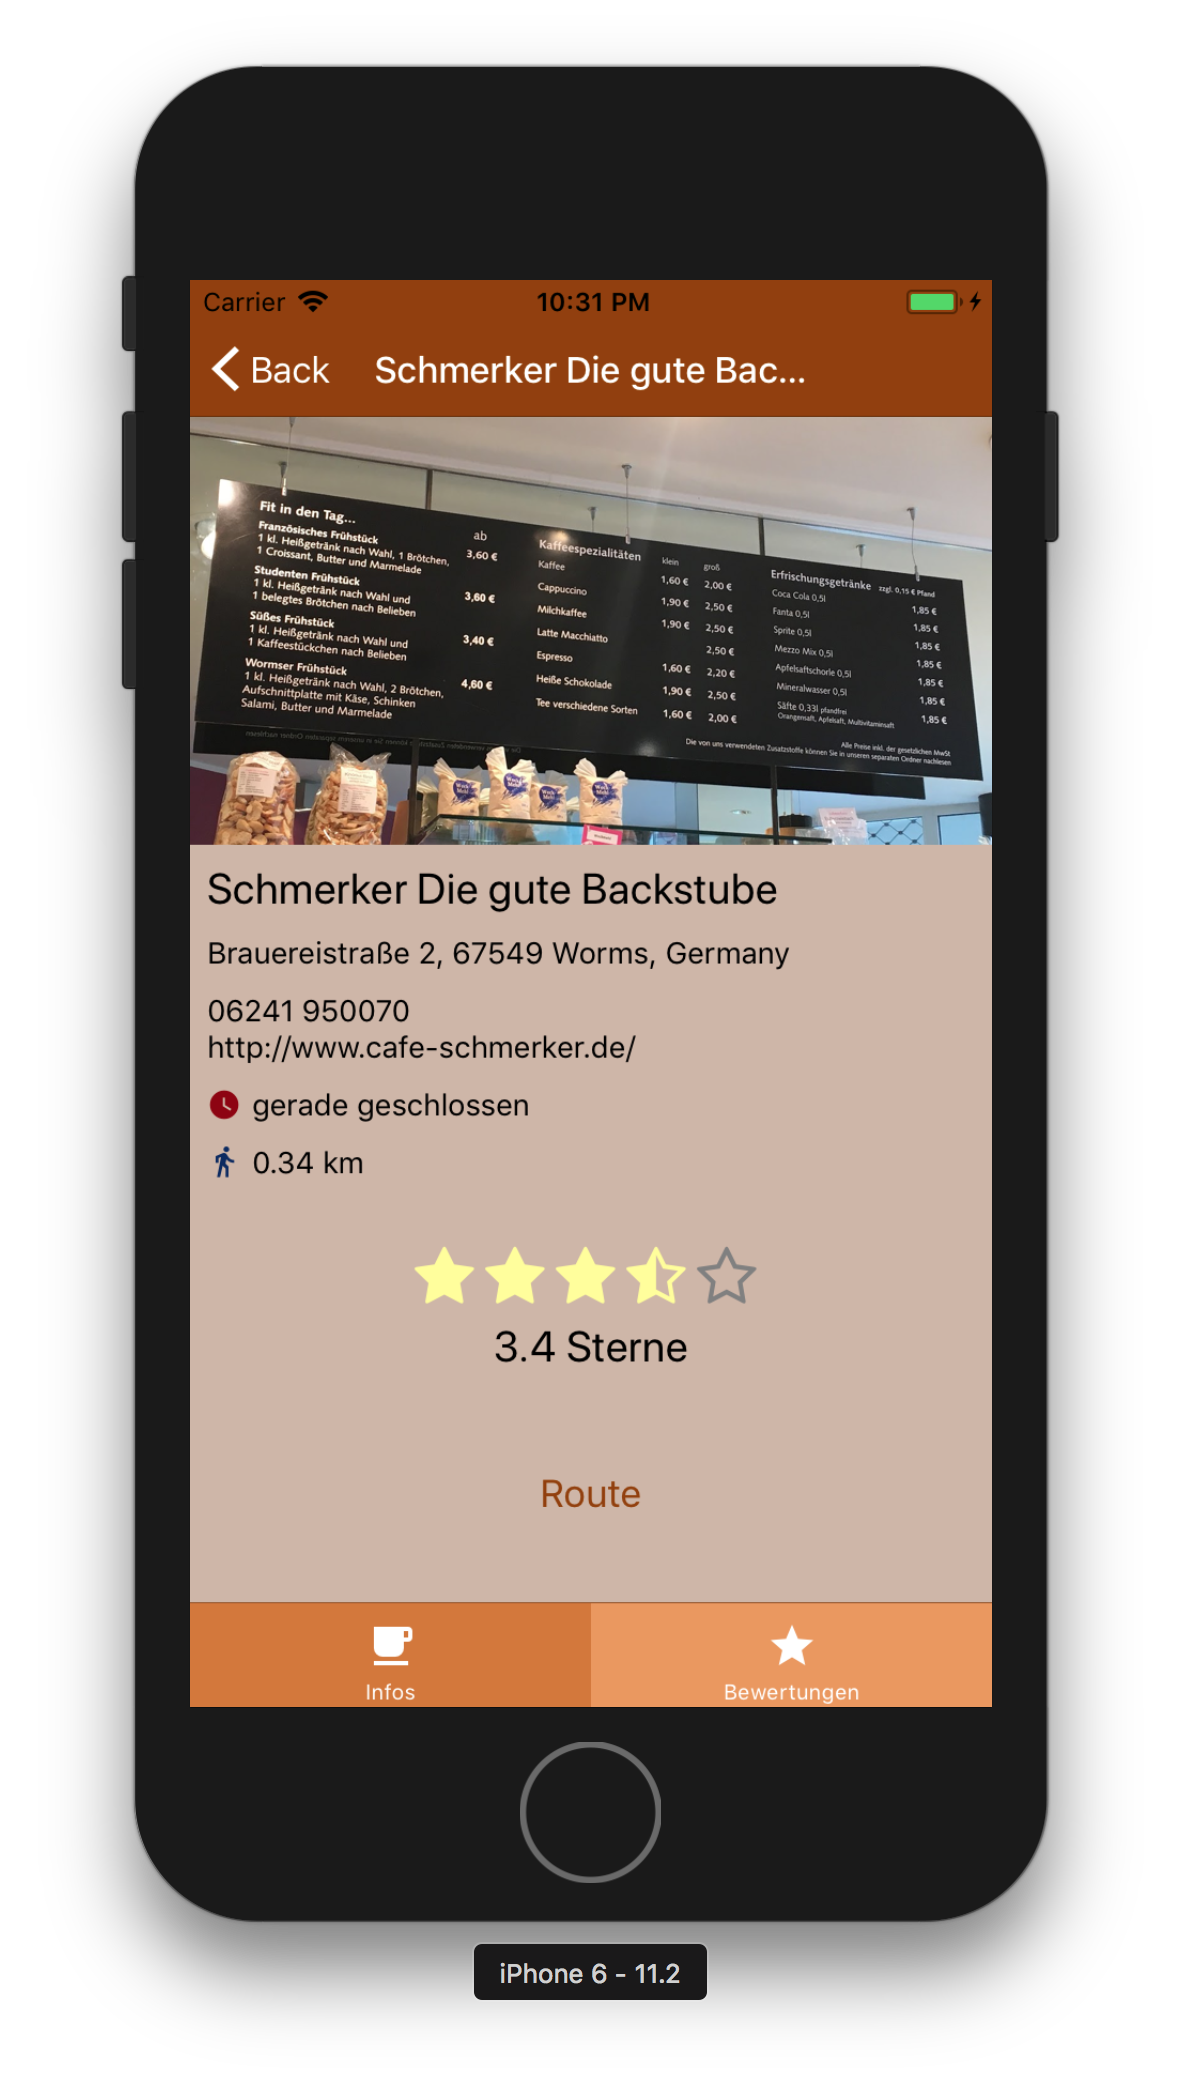
\includegraphics[width=0.5\textwidth]{Bilder/app-info.png}
		\captionof{figure}{Infoseite eines Cafés der App unter iOS}
		\label{fig:infoios} &
		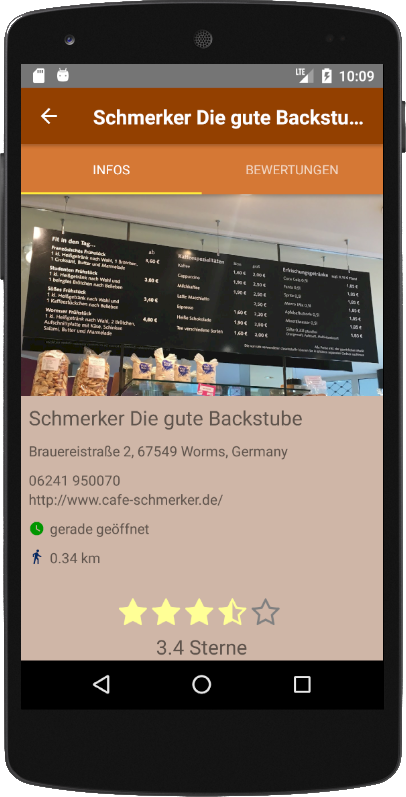
\includegraphics[width=0.48\textwidth]{Bilder/app-info_android.png}
		\captionof{figure}{Infoseite eines Cafés der App unter Android}
		\label{fig:infoandroid}
	\end{tabular}
\end{table}

\begin{table}
	\vskip-4.0cm\hskip-0.2cm\begin{tabular}{p{0.5\textwidth}p{0.5\textwidth}}
		\multicolumn{2}{p{\textwidth}}{\subsection{Bewertungen Café}} \\
		\multicolumn{2}{p{\textwidth}}{Alle über die Google API verfügbaren Bewertungen des ausgewählten Cafés werden hier in einer Liste angezeigt. Dabei erhält man Infos wie den Wert der abgegebenen Bewertung, den Zeitraum, den Bewertungsext sowie den Namen des Re­zen­senten (vgl. Abb. \ref{fig:bewertungios} und \ref{fig:bewertungandroid}).\newline} \\
		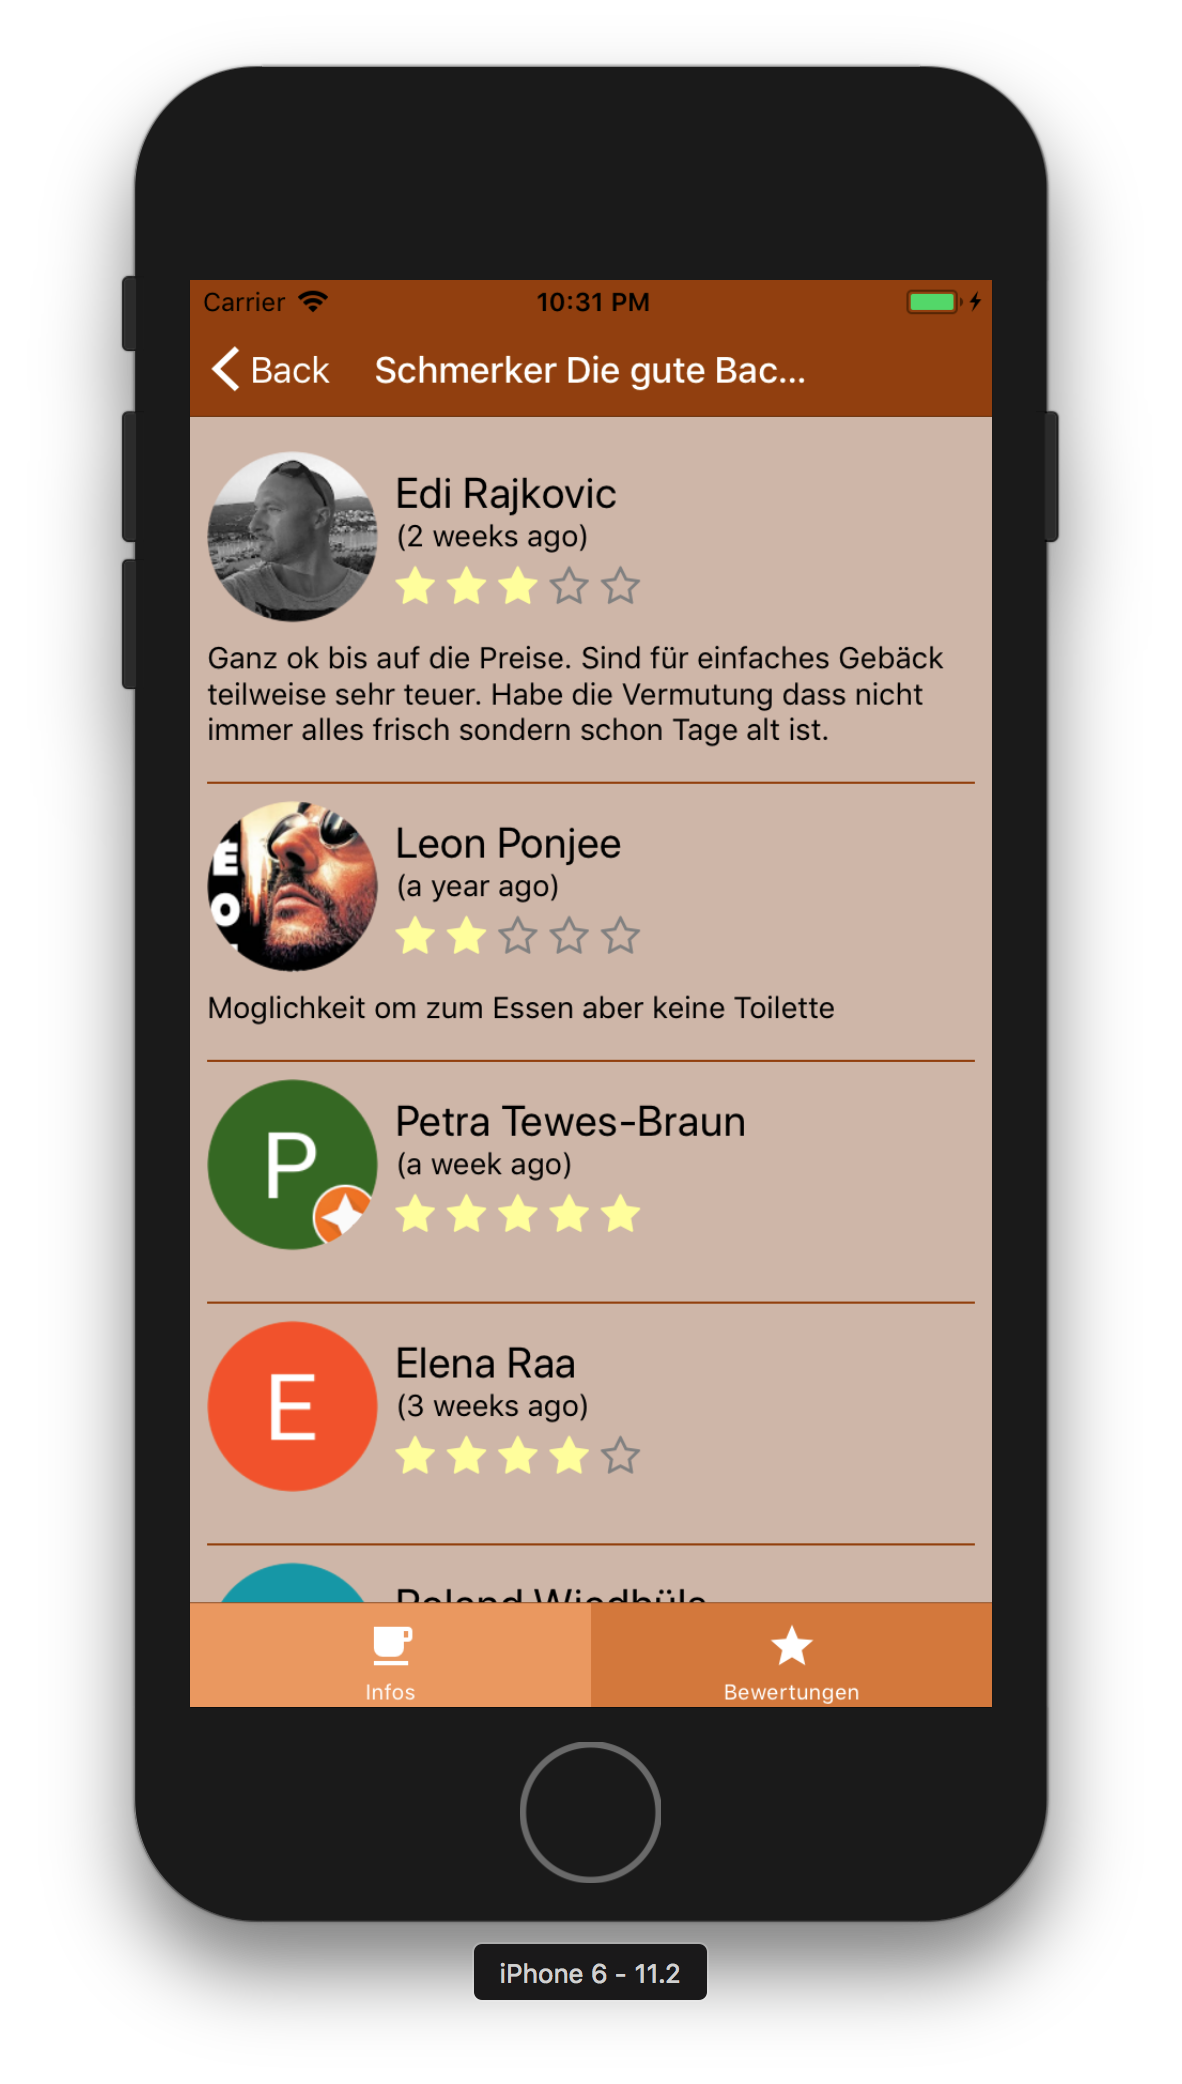
\includegraphics[width=0.5\textwidth]{Bilder/app-bewertungen.png}
		\captionof{figure}{Bewertungsseite eines Cafés der App unter iOS}
		\label{fig:bewertungios} &
		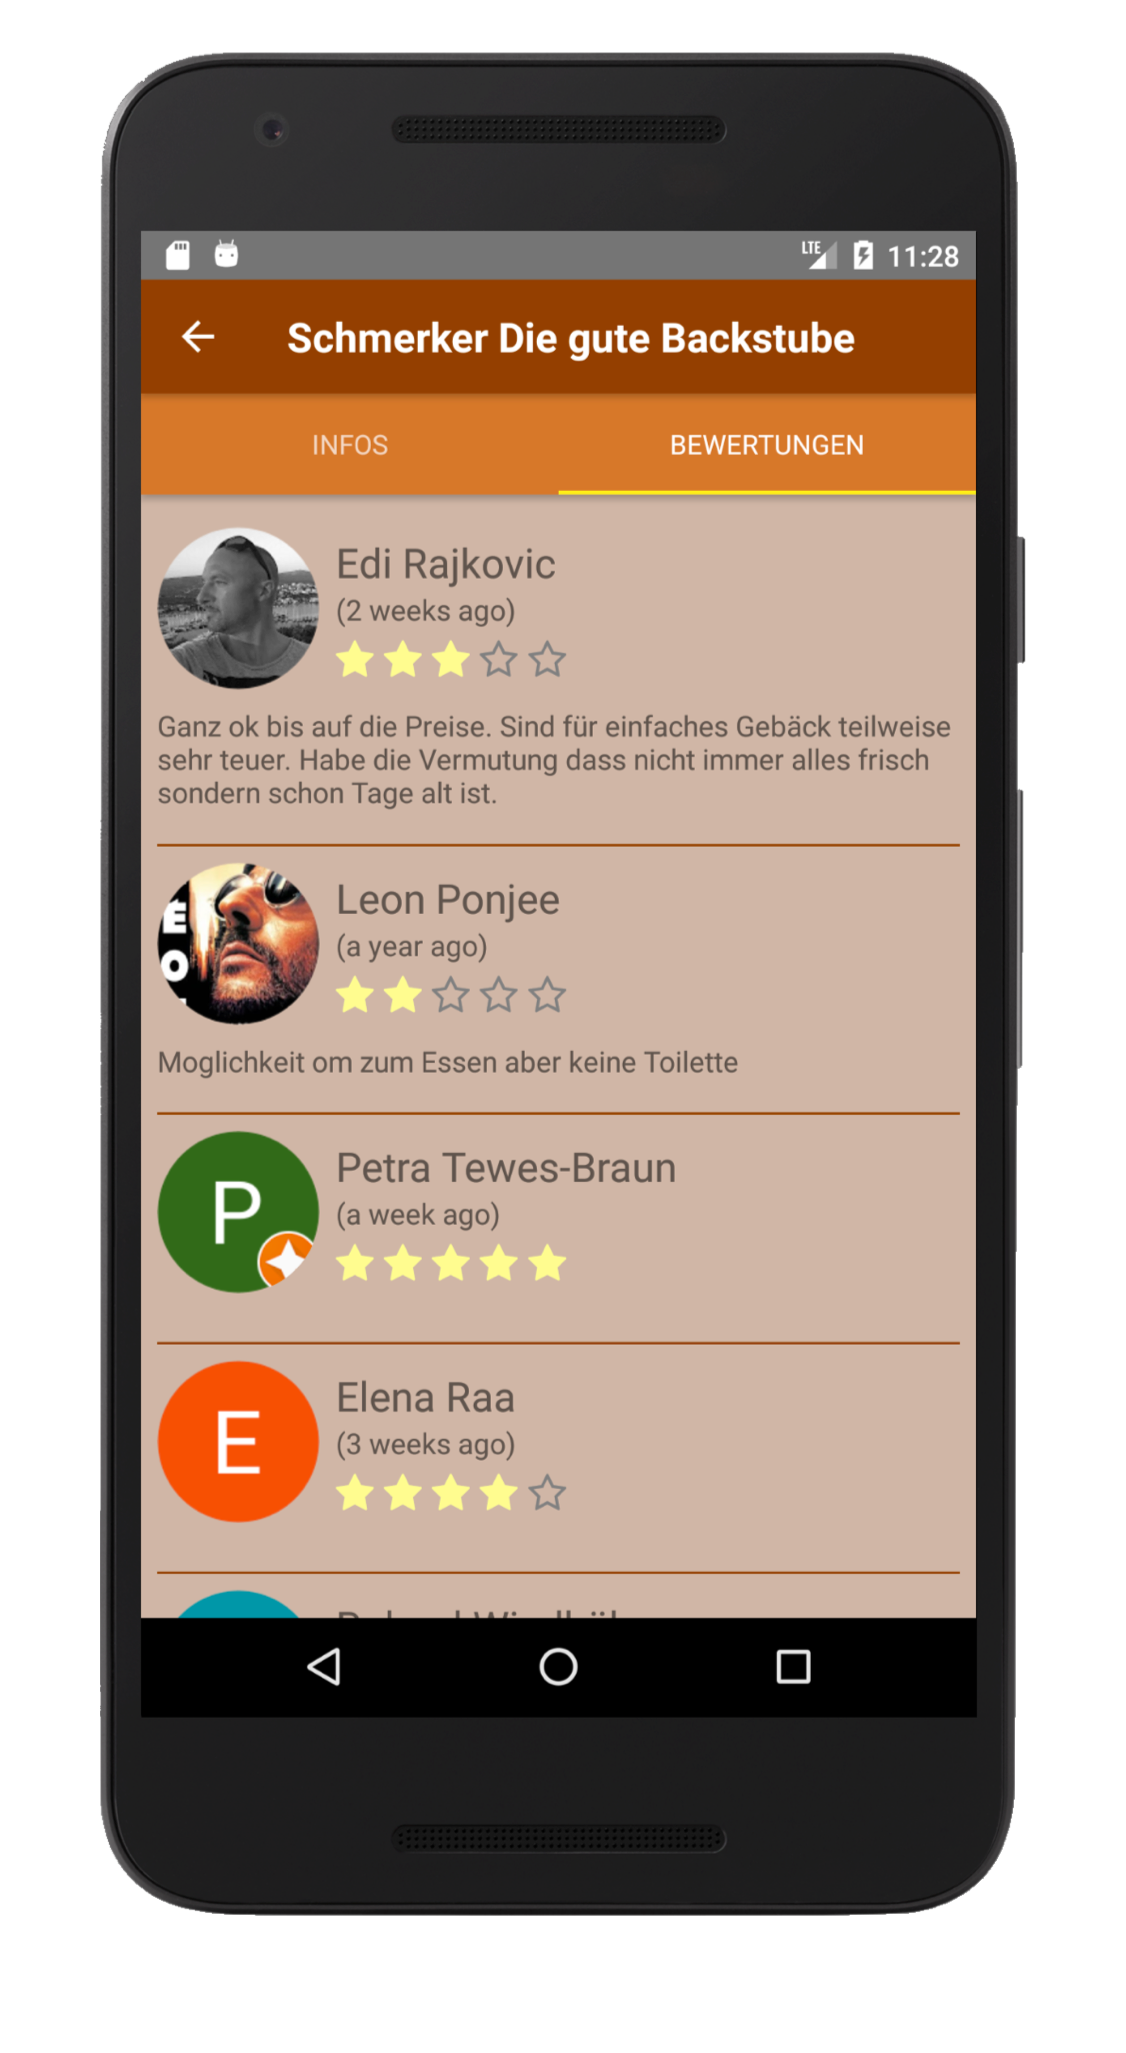
\includegraphics[width=0.48\textwidth]{Bilder/app-bewertungen_android.png}
		\captionof{figure}{Bewertungsseite eines Cafés der App unter Android}
		\label{fig:bewertungandroid}
	\end{tabular}
\end{table}

\begin{table}
	\vskip-3.0cm\hskip-0.2cm\begin{tabular}{p{0.5\textwidth}p{0.5\textwidth}}
		\multicolumn{2}{p{\textwidth}}{\subsection{Lexikon}} \\
		\multicolumn{2}{p{\textwidth}}{Die Übersichtsseite des Lexikons zeigt alle in der App hinterlegten Zubereitungsarten mit Namen und Icon (vgl. Abb \ref{fig:lexikonios} und \ref{fig:lexikonandroid}). Ein Klick auf eines dieser Elemente führt auf die zugehörige Detailseite (vgl. Kapitel \ref{subsec:detail}). Außerdem ist dies die einzige Seite, auf welcher der Bewegungssensor aktiv ist. Wird eine Schüttelgeste ausgeführt, so wird eine zufällig ausgewählte Zubereitungsart in einem Alert angezeigt. Von diesem aus kann man ebenfalls entweder direkt zur vorgeschlagenen Detailseite gelangen oder den Alert wieder entfernen.\newline} \\
		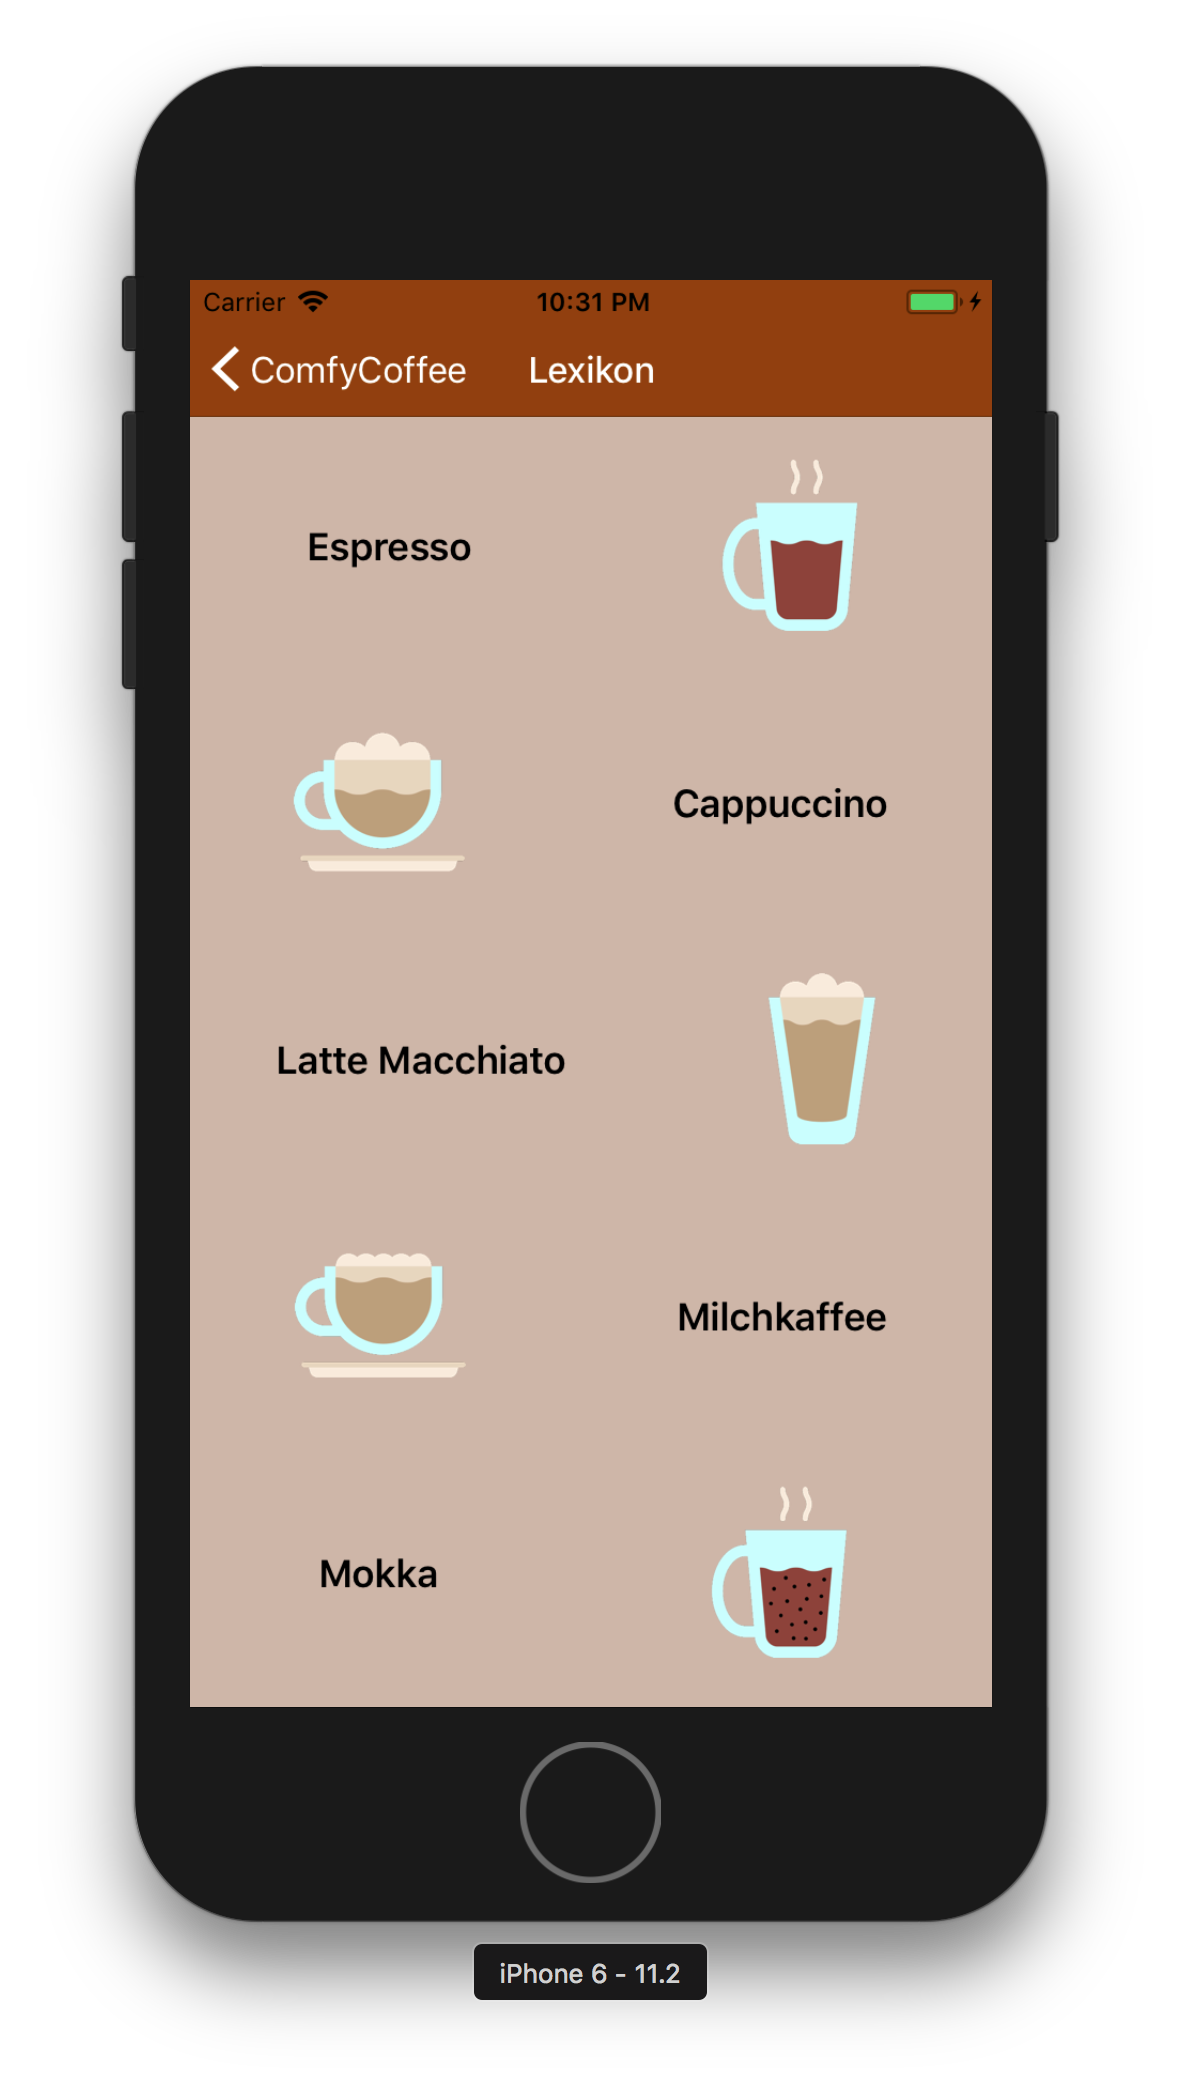
\includegraphics[width=0.5\textwidth]{Bilder/app-lexikon.png}
		\captionof{figure}{Lexikonseite der App unter iOS}
		\label{fig:lexikonios} &
		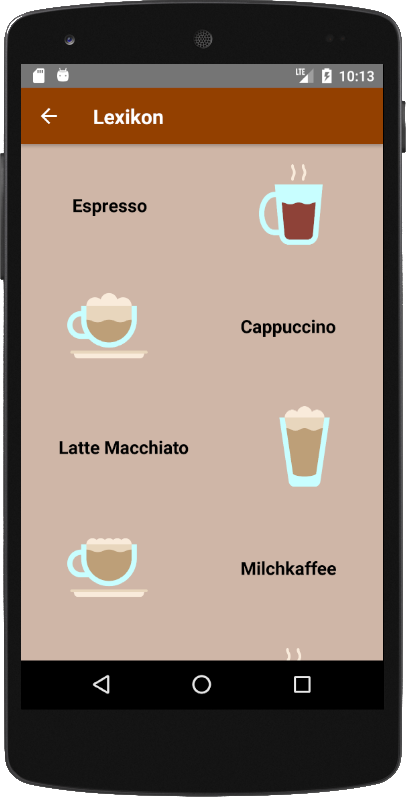
\includegraphics[width=0.48\textwidth]{Bilder/app-lexikon_android.png}
		\captionof{figure}{Lexikonseite der App unter Android}
		\label{fig:lexikonandroid}
	\end{tabular}
\end{table}

\begin{table}
	\vskip-3.5cm\hskip-0.2cm\begin{tabular}{p{0.5\textwidth}p{0.5\textwidth}}
		\multicolumn{2}{p{\textwidth}}{\subsection{Lexikon Detailansicht}\label{subsec:detail}} \\
		\multicolumn{2}{p{\textwidth}}{Hat man sich für eine Zubereitungsart entschieden, erscheint das Template dieser Seite gefüllt mit den passenden Informationen. Dazu gehören der Name, das Icon, eine Beschreibung des Ablaufs sowie einige Attribute wie Stärke des Getränks oder Menge des benötigten Wassers. Diese Informationen sind an die jeweils ausgewählte Zubereitungsart angepasst (vgl. Abb \ref{fig:lexikondetailios} und \ref{fig:lexikondetailandroid}).\newline} \\
		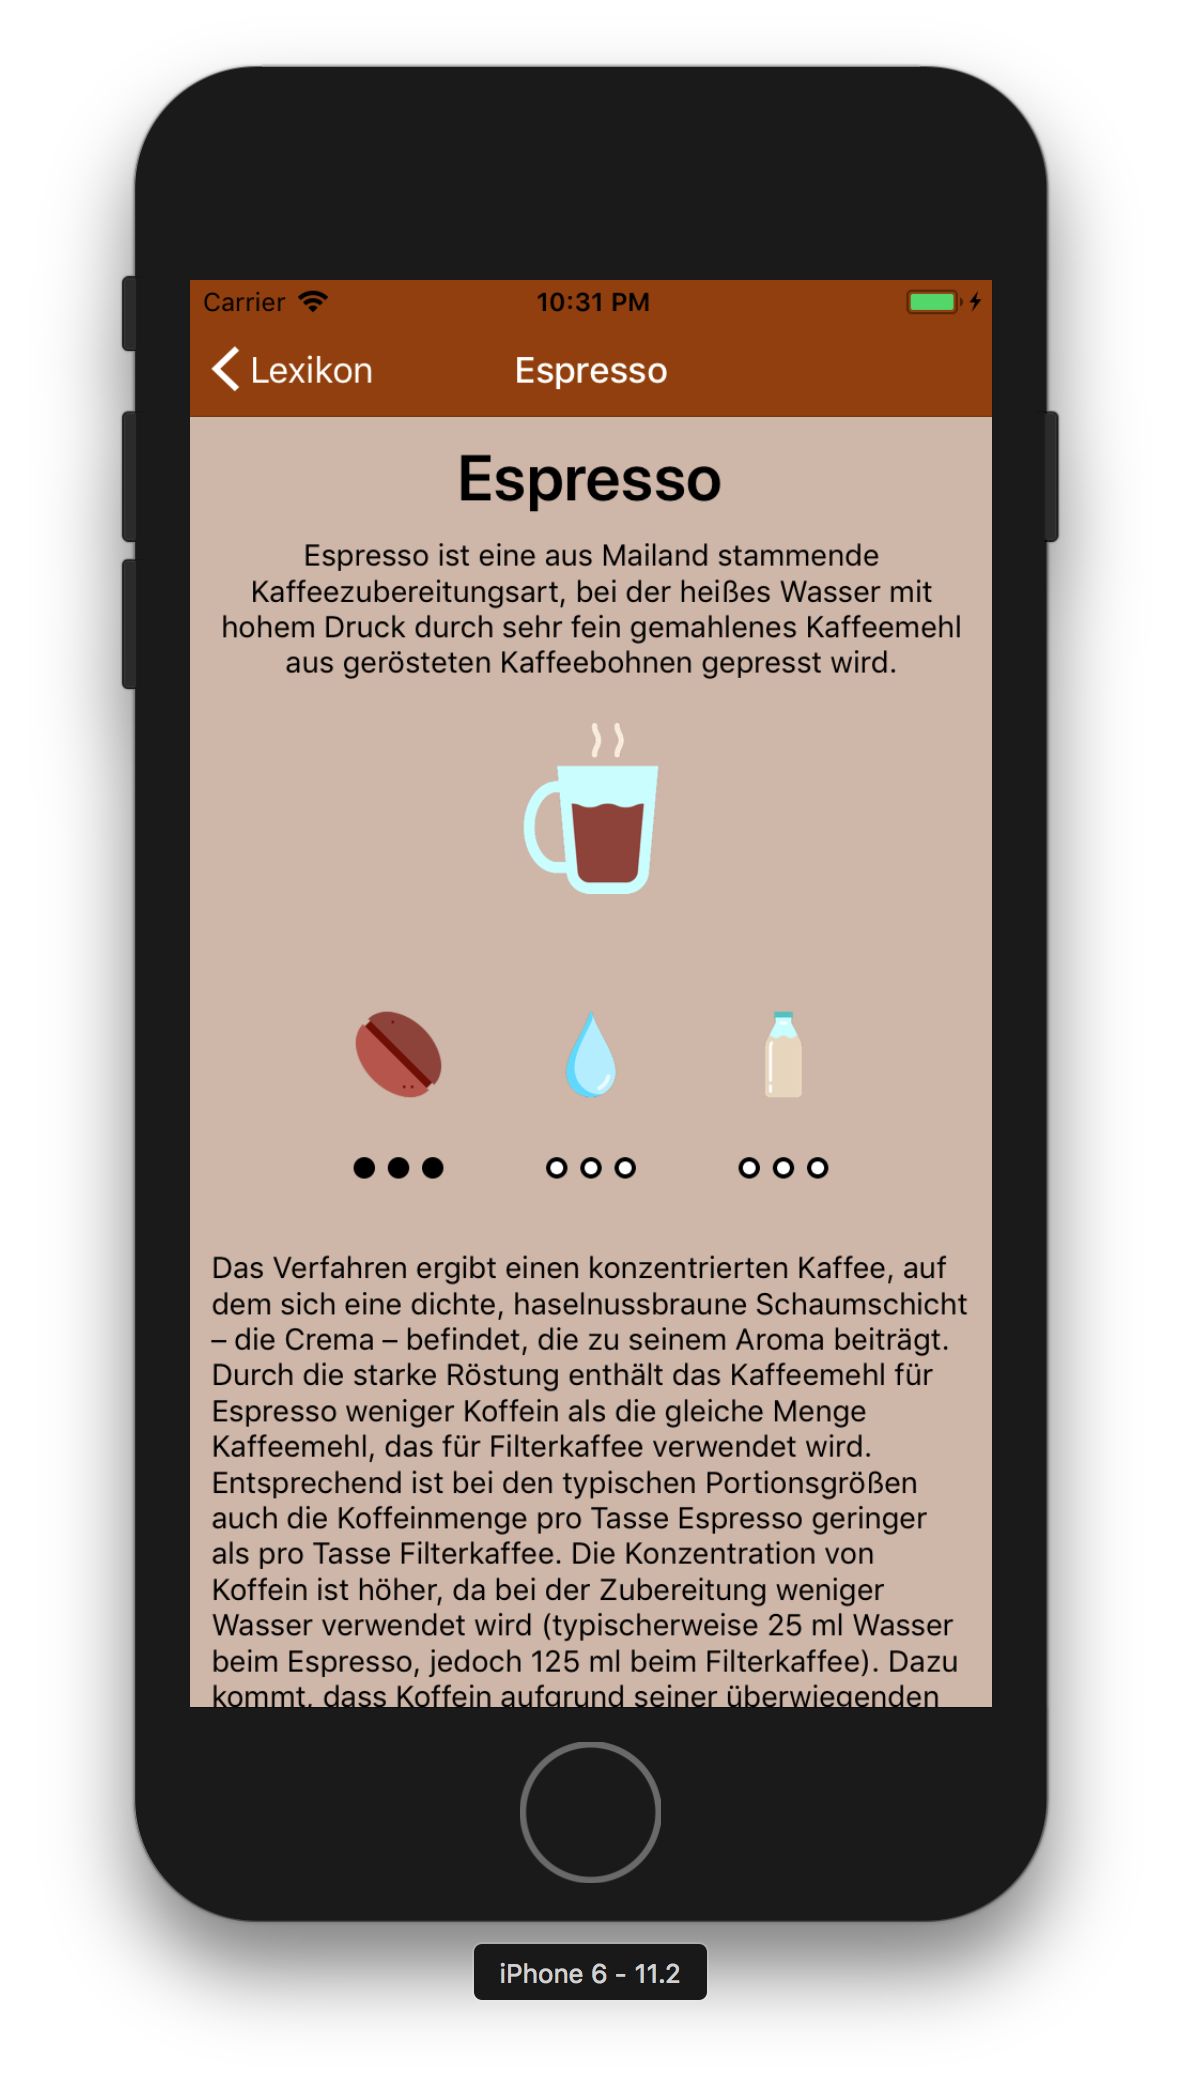
\includegraphics[width=0.5\textwidth]{Bilder/app-lexikon-detail.png}
		\captionof{figure}{Detailansicht eines Lexikoneintrags der App unter iOS}
		\label{fig:lexikondetailios} &
		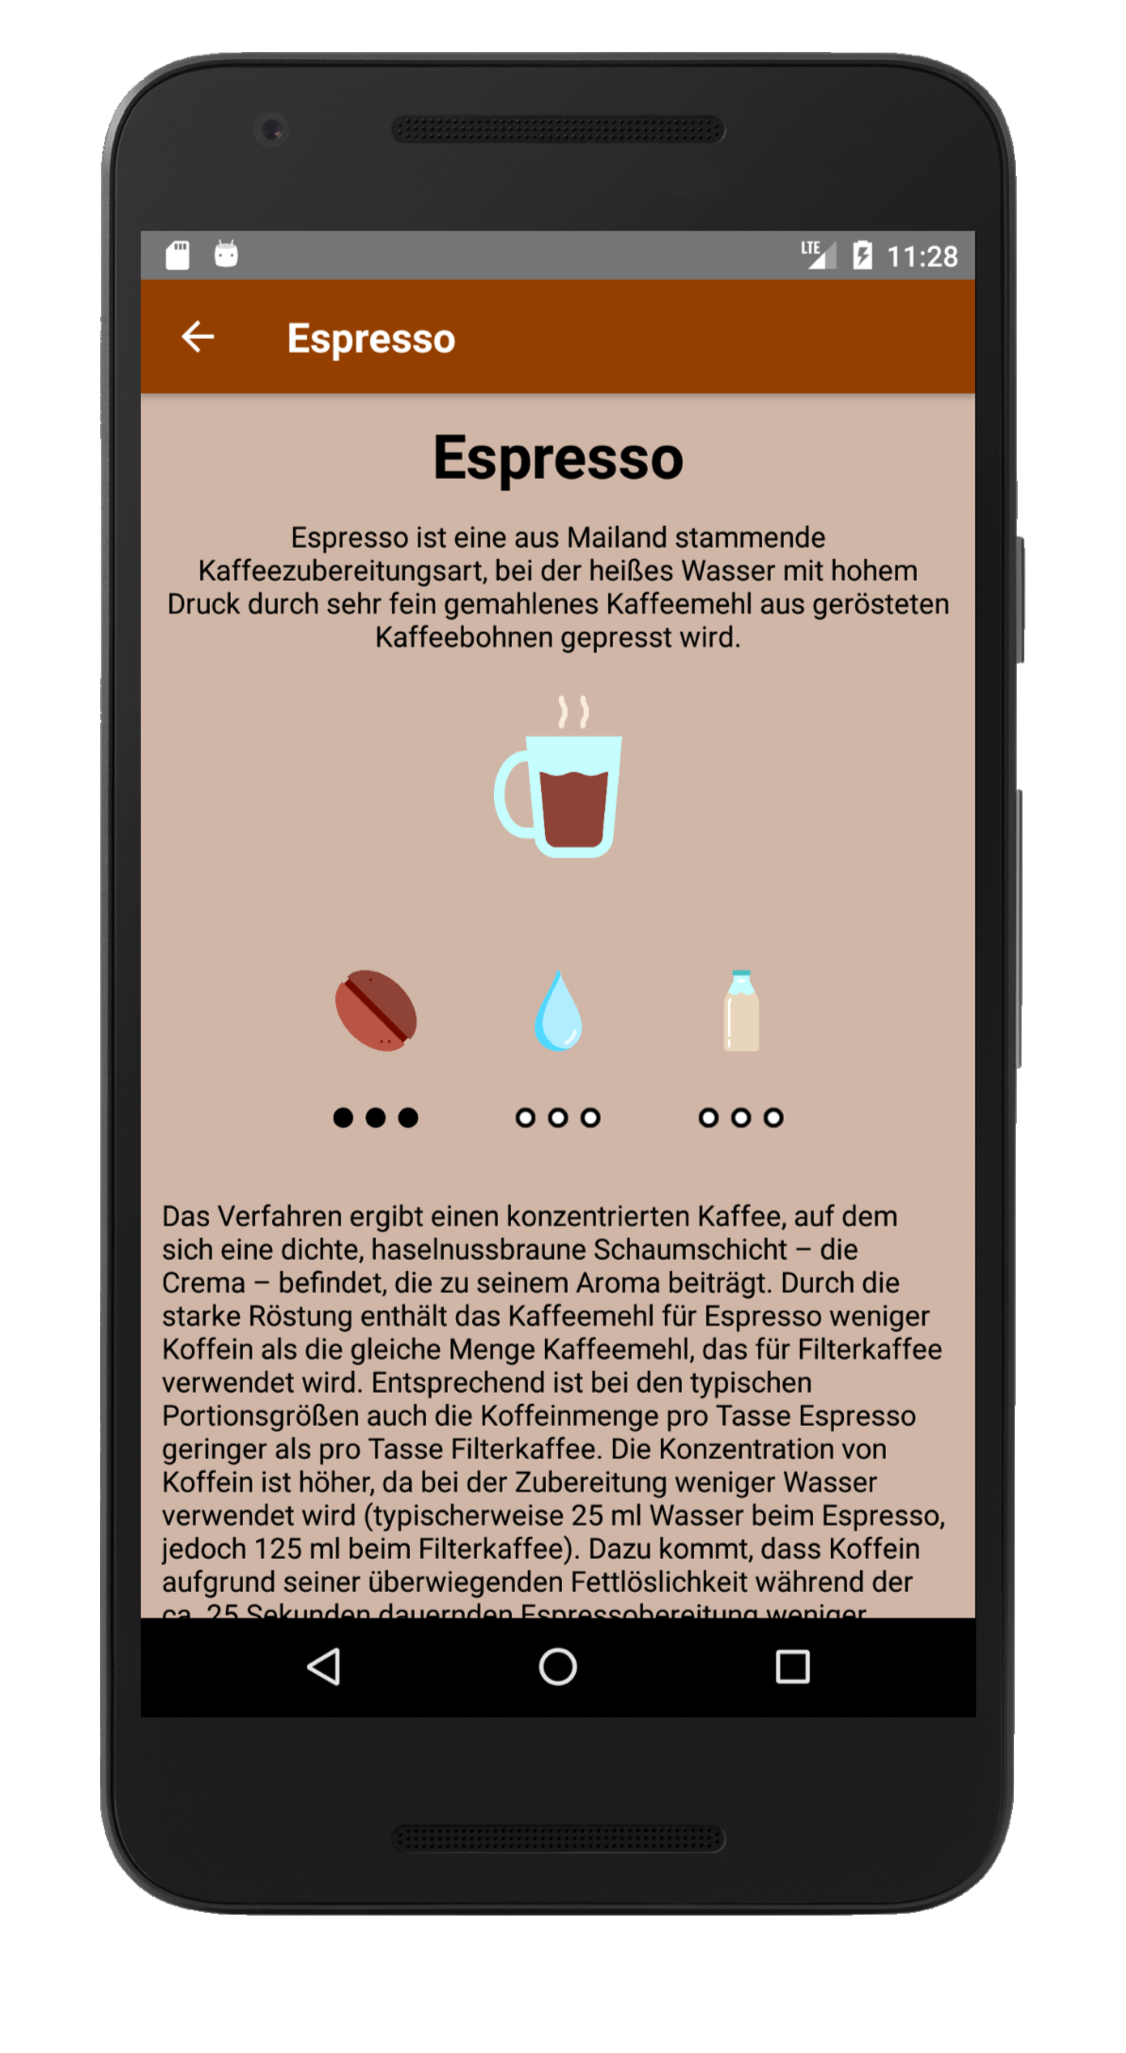
\includegraphics[width=0.48\textwidth]{Bilder/app-lexikon-detail_android.png}
		\captionof{figure}{Detailansicht eines Lexikoneintrags der App unter Android}
		\label{fig:lexikondetailandroid}
	\end{tabular}
\end{table}


\newpage

\section{Readme}
comfycoffee ist eine Cross-Plattform App zur Anzeige lokaler Cafés und damit nachhaltigen Unterstützung der lokalen Kaffeewirtschaft.
Das Repository ist öffentlich und unter folgendem Link erreichbar: \url{https://bitbucket.org/codemeleon/comfycoffee}.
Das Projekt ist lizensiert unter der MIT Lizenz.

Weitere Informationen können der offiziellen React Native Dokumentation entnommen werden.

\subsection{Voraussetzungen}
Um an dem Projekt zu arbeiten müssen folgende Tools installiert sein:

\begin{itemize}
	\item node.js (v8.6.0 wird empfohlen)
	\item npm (v5.3.0 wird empfohlen)
	\item Watchman
	\item Xcode (für iOS Builds - nur für MacOS)
	\item Android Studio (für Android Builds)
\end{itemize}

Es wird die Verwendung von \emph{Visual Studio Code (VS Code)} als Code Editor empfohlen.
Das VS Code Plugin \emph{Prettier - Code formatter} sorgt hierbei für einen sauber formatierten Code. Weiterhin muss eine Verbindung mit dem Internet bestehen, um das Projekt bauen zu können.

\subsection{Testing und Debugging}
Das Testing und Debugging kann über die in Android Studio und Xcode integrierten Simulatoren erfolgen.
Eine weitere Möglichkeit ist die direkte Verbindung zu einem Smartphone/iPhone über USB.
Wird ein derartiges Endgerät erkannt erfolgt die Kompilierung direkt auf das Gerät.
Hilfreiche Freatures wie JavaScript Debugging im Browser oder LiveReload können direkt im Simulator oder auf dem Endgerät aktiviert werden.

Relevante Befehle in der Kommandozeile sind hierbei:\\
\emph{react-native run-andoid}\\
\emph{react-native run-ios}






\chapter{Ausblick}
\label{ausblick}
Während und nach der Entwicklung sollen Tests sicher stellen, dass die App gut bedienbar ist. Das Testkonzept hierfür wird in Kapitel \ref{sec:testkonzept} erläutert.

Anschließend spielt das Marketing eine wichtige Rolle, um die App erfolgreich unter die Zielgruppe zu bringen. Ansätze und Ideen hierfür sind in Kapitel \ref{sec:marketing} dargelegt.

\section{Testkonzept}
\label{sec:testkonzept}
Das Testkonzept besteht aus einem \emph{Usability Test}, der zusätzlich ein \emph{Interview} und einen \emph{A/B-Test} beinhaltet.

Für den Usability Test werden 10 bis 20  Versuchsteilnehmer aus der Zielgruppe benötigt. Unter Beobachtung sollen sie die App bedienen und mit ihr bestimmte Aufgaben lösen. Währenddessen sollen die Teilnehmer laut aussprechen, was sie gerade denken und tun (\emph{Thinking Aloud}). So lassen sich unlogische Abläufe und unklare Bedienungen in der App herausfinden.

Das Interview wird als halb-strukturiertes Interview durchgeführt. Offene Fragen, die sich auf die App im Allgemeinen beziehen, lassen der Versuchsperson die Freiheit, ihre ganz persönlichen Eindrücke wiederzugeben. Diese Ergebnisse sind schwer zu vereinheitlichen und müssen mit entsprechender Umsicht behandelt werden, da sie sehr subjektive Empfindungen beinhalten, die sich unter Umständen nicht mit einem Großteil der Zielgruppe decken. Es muss stets abgewogen werden, ob und wie die Ergebnisse der offenen Fragen umgesetzt werden. Der geschlossene Teil des Interviews bezieht sich auf den A/B-Test im folgenden Abschnitt.

Beim A/B-Test wird ein Bestandteil der App in zwei unterschiedlichen Ausführungen getestet. Die Versuchspersonen werden in zwei Gruppen aufgeteilt, eine Gruppe erhält die App mit dem Bestandteil in der Version A, die andere die gleiche App, die sich nur darin unterscheidet, dass Bestandteil A durch B ausgetauscht wird. Im Fall von comfycoffee wäre zu testen, in welcher Form die Schüttelfunktion besser bei der Zielgruppe ankommt. Ursprünglich weist die Schüttelfunktion den Nutzer auf eine zufällige Kaffeesorte hin (vgl. Kapitel \ref{subsec:mussanforderungen}). Eine weitere Idee ist, über die Schüttelfunktion zufällig auszuwürfeln, wer von zwei oder mehreren Nutzern den Kaffee bezahlt. Präzise geschlossene Fragen sollen darüber Auskunft geben, welche Funktion von der Zielgruppe besser angenommen wird.

\underline{Learnings:}
Auch nach der Entwicklung ist noch viel zu tun. Regelmäßiges Testen erhöht die Usability der App und bringt den Entwickler auf den Boden der Tatsachen zurück.

\section{Marketing}
\label{sec:marketing}
Beim Marketing wurden die Bereiche \emph{Produktpolitik}, \emph{Preispolitik}, \emph{Distributionspolitik}, \emph{Kommunikationspolitik} und \emph{Retention Marketing} ausgearbeitet. Anhand von Analysetools, wie beispielsweise \emph{Google Analytics}, können Statistiken zur App-Nutzung erfasst werden, anhand derer die App ausgewertet und weiter verbessert werden kann.

\underline{Learnings:}
Marketing ist ein eigenes Themengebiet mit vielen Facetten, die es zu meistern gilt, um eine App wirkungsvoll unter die Zielgruppe zu bringen. Hier wird viel Einarbeitung und Ausdauer verlangt, um erfolgreich zu sein.

\subsection{Produktpolitik}
comfycoffee wird als Cross-Plattform App für Android und iOS entwickelt. Eine zusätzliche Web-App für Desktopnutzer ist denkbar.

\subsection{Preispolitik}
comfycoffee wird als kostenfreier Download in den App-Stores zur Verfügung stehen. Cafés können einen höheren Platz in der Listenansicht der Cafés erkaufen, diese Einträge werden für den Nutzer kenntlich mit ``Anzeige'' markiert. Mit den Daten der Nutzer sowie der Cafés kann personalisierte Werbung innerhalb der App geschaltet werden.

Eine weitere Idee wäre, die App für einen geringen Preis in die App-Stores zu stellen. Dem Nutzer wird der Kauf schmackhaft gemacht, indem er Gutscheine von Cafés durch die App erhält, welche die Kosten für die App wieder aufwiegen.

\subsection{Distributionspolitik}
Die App wird in den App-Stores (\emph{Google Play} für Android und \emph{App Store} für iOS) sowie über den Browser (Web-App) zur Verfügung gestellt.

\subsection{Kommunikationspolitik}
Eine dedizierte Landing-Page ist die erste Anlaufstelle für comfycoffee. Weitere Social Pages dienen ebendiesem Zweck. Durch Social Media Werbung, besonders in ``Support your Locals''-Communities und durch Influencer, soll die Bekanntheit der App gesteigert werden.

Ein eigener Blog soll die Nutzer informieren und neue Nutzer gewinnen. Ein ``Kaffee-Reporter'' fungiert als Gesicht für die App und stellt Themen wie der ``Coffee of the Week'', die ``Location of the Week'' oder aktuelle Kaffee-Trends vor.

Offline-Werbung in Cafés vor Ort und in Zeitungen machen die App auch in Kreisen bekannt, die weniger in den Soziale Medien unterwegs sind.

\subsection{Retention Marketing}
comfycoffee soll die Nutzer motivieren, die App regelmäßig zu nutzen. Hierfür können mit den Cafébesitzern, deren Cafés in der App aufgelistet werden, Gutscheine ausgehandelt werden, welche die Nutzer über die App erhalten und einlösen können.

Die Nutzer können durch den Besuch ihres Lieblingscafés Punkte erhalten, anhand derer sie in einer Rangliste nach oben steigen können. Die Top 10 der Besucher des jeweiligen Cafés werden in der App aufgelistet. Alternativ können die Nutzer Punkte erlangen, indem sie möglichst viele verschiedene Cafés besuchen. Durch diese Art der Gamification sollen die Nutzer Spaß an der App haben und diese durch den Ehrgeiz der Punktegewinnung möglichst oft nutzen.

Innerhalb der App kann auf bestimmte seltene Kaffeesorten aufmerksam gemacht werden, z. B. wenn sich der Nutzer gerade in der Nähe eines Cafés befindet, welches diese Sorte anbietet. Aktuelle Kaffee-Trends können zeitlich begrenzt in der App angesehen werden. Durch den Besuch eines Cafés können weitere Einträge im Lexikon freigeschaltet werden. Eine zeitliche Limitierung dieser Einträge fordert den Nutzer dazu auf, comfycoffee häufig zu nutzen.